\documentclass[twocolumn]{article}

\usepackage{geometry}
\geometry{textwidth = 18cm,textheight = 24cm}

\usepackage[utf8]{inputenc}
\usepackage{multirow}
\usepackage{graphicx}
\usepackage{outlines}
\usepackage[dvipsnames]{xcolor}
\usepackage{textcomp}
\usepackage{float}
\usepackage{ulem}
\usepackage{comment}

\usepackage{hyperref}
\hypersetup{
    citecolor = red,
    filecolor = green,
    urlcolor = orange,
    colorlinks = true, %set true if you want colored links
    linktoc = all,     %set to all if you want both sections and subsections linked
    linkcolor = blue,  %choose some color if you want links to stand out
}

%\title{Comparison of semiconductor and superconductor hardware for large-scale optoelectronic neural systems}
\title{\textcolor{OliveGreen}{Considerations for neuromorphic supercomputing in semiconducting and superconducting optoelectronic hardware}}
\author{Bryce A. Primavera and Jeffrey M. Shainline}
\date{March 2021}

\begin{document}

\twocolumn[
\begin{@twocolumnfalse}
\maketitle
\begin{abstract}
Any large-scale neuromorphic system striving for complexity at the level of the human brain and beyond will need to be co-optimized for communication and computation. Such reasoning leads to the proposal for optoelectronic neuromorphic platforms that leverage the complementary properties of optics and electronics. Optical communication allows for direct connections between neurons, which removes bottlenecks associated with network traffic. Electronic computation allows for complex synaptic and neuronal functions. Starting from the hypothesis \textcolor{red}{(conjecture?)} that future large-scale neuromorphic systems will utilize integrated photonics and fiber optics for communication in conjunction with electronics for computation, we consider two possible paths towards achieving this vision. The first is a semiconductor platform based on analog CMOS circuits and waveguide-integrated photodiodes. The second is a superconducting approach that utilizes Josephson Junctions \sout{(JJs)} \textcolor{red}{(let's try to avoid introducing acronyms until the main text)} and waveguide-integrated superconducting \sout{nanowire} single-photon detectors \sout{(SNSPDs)}. We argue that these two systems can \textcolor{ForestGreen}{both} implement \sout{similar} \textcolor{ForestGreen}{adequate} synaptic and neuronal dynamics. With this established, the two platforms are analyzed from several viewpoints: power consumption, speed, area, \sout{available} memory\textcolor{ForestGreen}{/plasticity} \sout{technologies}, cooling, and \sout{feasibility of} fabrication. While both platforms require significant technological innovations to become viable, we reach some early conclusions about their limits and device performance metrics that will \sout{likely} need to be met for optoelectronic neuromorphic supercomputers to become a useful paradigm. Notably, it is found that the minimum possible energy used for communicating events is likely to be of the same order in both cases, but the superconducting approach dramatically lessens the optical power required of the integrated light-sources, which remain the most speculative element of both platforms. An ideal neuromorphic platform also possesses local memory integrated within synaptic circuits. While synaptic circuits with activity-based plasticity mechanisms have seen great progress in recent years, learning functionality is still left wanting. Superconducting electronics introduces new, but rather unexplored paths for integrated memory that appear promising for synaptic adaptation based on the same signals used elsewhere in the network for communication and computation. Lastly, the physical, system-level instantiation of massive optoelectronic networks is considered for both cases, including cooling systems, area considerations, and the importance and prospects of 3D integration. Superconducting systems appear more naturally suited for 3D integration due to room-temperature processing. While this study cannot determine which nascent platform will be superior in the future, it enumerates a list of technological advances that will be required if either approach is going to achieve its lofty ambitions \sout{and identifies major concerns}. \textcolor{ForestGreen}{Our intention is for the list of necessary advances to aid the} community \sout{to accurately} in assessing the progress of both platforms \sout{in future years} and to \sout{maintain a focus on systems that will be truly scalable} \textcolor{ForestGreen}{direct attention to unique aspects of optoelectronic systems that become significant in the unique context of large-scale neural systems}. \textcolor{red}{(I think the abstract is strong, maybe a tad long)}
\vspace{2em}
\end{abstract}
\end{@twocolumnfalse}
]

\setcounter{tocdepth}{4}
\setcounter{secnumdepth}{4}
\tableofcontents

\section{\label{sec:introduction}Introduction}

The foundations of cognition remain a great frontier of science, with potentially enormous ramifications for technology and society. A platform capable of simulating neural function on the scale of the brain and beyond could be a powerful tool in unravelling these great mysteries. Achieving \sout{that scale, however,} \textcolor{ForestGreen}{such large-scale systems has proven to be non-trivial with established CMOS hardware \cite{}.}  \sout{will likely require new architectures and the development of novel hardware.} A significant challenge will be to construct systems that enable efficient communication with low-latency amongst billions or trillions neurons. Optical communication appears well-matched to the task, as the lack of resistive, capacitive, and inductive parasitics makes optical links more amenable to high fan-out as compared to electrical interconnects \cite{shainline2018largest}. In the present work, \textcolor{ForestGreen}{we take the premise of optical communication with electronic computation as the starting point for the design of large-scale neural systems, and we attempt to anticipate some of the challenges that may arise related to functionality, power consumption, and fabrication. In this context, we use the term ``large-scale'' to refer to systems with $10^{10}$ neurons or more, where this number is chosen somewhat arbitrarily, as it is the number of neurons in the human cerebral cortex.} \sout{we consider aspects of optoelectronic hardware that must be considered if brain-scale systems are to be achieved.}

To date, most neuromorphic systems are fabricated in standard CMOS processes and make use of a digital communication infrastructure called Address Event Representation (AER, \cite{bo2000,payu2017}). AER uses an addressing system to time-multiplex spiking events from many neurons on to a small number of buses in order to circumvent the physical issues that limit CMOS circuits to only a handful of outputs. This framework has been very successful \textcolor{ForestGreen}{in overcoming physical fan-out limitations,} and neuromorphic chips \textcolor{ForestGreen}{leveraging AER and} targeting edge \textcolor{red}{(do we need to define ``edge''?)} applications are beginning to be commercialized \cite{merolla2014million, davies2018loihi} \textcolor{red}{(are these two chips being commercialized? is commercialization the focus?)}. Additionally, their programmability and \sout{accessibililty} \textcolor{ForestGreen}{reconfigurability} make them valuable tools for testing testing hypotheses in neuroscience and artificial intelligence. However, \textcolor{ForestGreen}{time multiplexing leverages the speed of CMOS systems to mitigate connectivity limits, and the result is a trade-off} \sout{multiplexing inherently introduces trade-offs} between connectivity, latency, \textcolor{ForestGreen}{and memory}. \textcolor{ForestGreen}{As the number of neurons and synapses in the network increases, larger memory is required to hold the address space, and accessing this memory becomes a more cumbersome aspect of system operation. As the total communication traffic on the network increases, hardware resources must be dedicated to arbitration of events simultaneously requesting access to the routing infrastructure. For all know communication networks based on a shared switching fabric, latency grows exponentially beyond a certain traffic level \cite{hepa2011}. Such traffic-dependent delays are a severe limitation to spiking neural networks, in which the timing of spikes contains important information \cite{}. AER has played a crucial role in enabling the development of CMOS neuromorphic systems, and further progress should be pursued. Nevertheless, in this work we consider the possibilities for neuromorphic hardware that may arise if AER is sidestepped by utilization of optical communication.} \sout{It is thus unclear if AER, and even electronic communication more broadly, will be the optimal solution for future neural systems pushing the limits of cognition.}

\textcolor{ForestGreen}{The objective when utilizing }optical communication is to eliminate the need for time-multiplexing, allowing direct, physical connections between neurons. Unlike electrons, photons do not interact strongly with each other, allowing for low cross-talk and high fan-out. Additionally, waveguides and optical fibers enable low-loss communication up to the scale of meters\textemdash an advantage commonly exploited by long-distance communication systems that has been increasingly applied to shorter and shorter length scales \cite{miller2017attojoule}. While the lack of interaction between photons is a benefit for communication, it is a detriment to computation. Electronic circuits are better suited to implement complicated, nonlinear neuronal functions. This has led to the hypothesis that the largest cognitive systems will be optoelectronic\textemdash utilizing optics for communication and electronics for computation \cite{shainline2018largest}. 

\textcolor{ForestGreen}{In the language commonly used in the neuromorphic engineering community, we seek fully dedicated axons for communication \cite{seda2016}. In this work we further specify that all synapses, dendrites, and neurons utilize fully dedicated circuits as well, so that each element of hardware has a one-to-one correspondence with its information-processing role in the neural system.} A number of concepts for \textcolor{ForestGreen}{fully dedicated} optoelectronic neuromorphic hardware have been proposed. In this paper, we will restrict ourselves to a discussion of \sout{only} two classes of networks (superconducting and semiconducting) designed around three basic assumptions:

%A variety of promising optoelectronic neuromorphic platforms have been proposed (\cite{shainline2019superconducting, nazirzadeh2018energy}), but here we limit the scope of the present study to systems that adhere to the following design rules:

\begin{enumerate}
    \item Direct connections are utilized \textcolor{ForestGreen}{(fully dedicated axons)}\sout{superior to shared connections}.
    \item Optical communication \textcolor{ForestGreen}{is} \sout{should be} binary. \textcolor{ForestGreen}{The amplitude of the optical signal carries no information.}
    \item All synaptic, dendritic, and somatic computations \sout{should be} are performed by \textcolor{ForestGreen}{(fully dedicated)} electronic circuits.
\end{enumerate}

\begin{figure*}
    \centering
    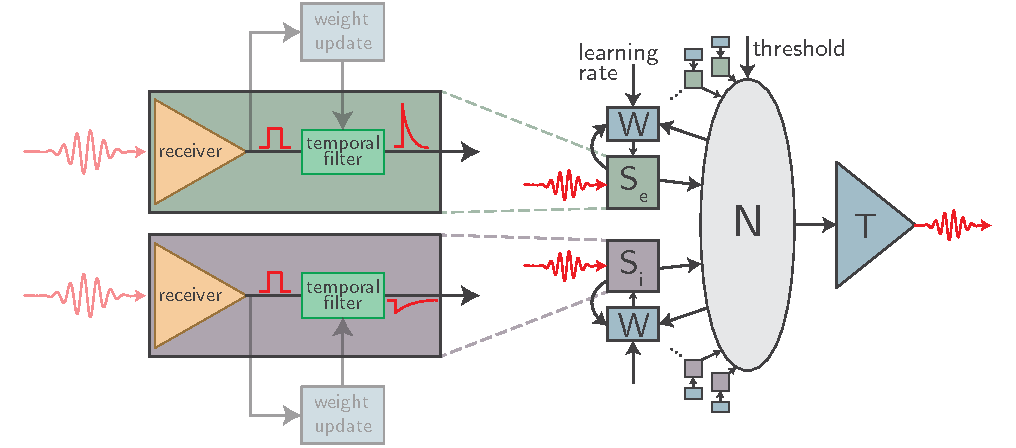
\includegraphics[scale=1]{_Schematic.pdf}
    \caption{An abstract schematic of the class of optoelectronic neurons meeting the three criteria given above. Each synapse ($S_e$ and $S_i$ for expiatory and inhibitory synapses respectively) is implemented with a physical circuit block containing a detector and a temporal filter. The detector produces an all-or-nothing electrical pulse upon receipt of an optical spike which is then processed by the filter. The parameters of the filter (time constant, weight, etc.) can be set individually for each synapse. A local weight update circuit (W) implements plasticity mechanisms at each synapse. Synaptic outputs are integrated in the soma (grey) which drives an optical transmitter to downstream connections upon reaching threshold.}
    \label{fig:Schematic}
\end{figure*}

These three conditions follow from the principles already mentioned. Optical communication is attractive precisely because it eliminates the need for shared communication lines by allowing for neurons with high fan-out. \sout{There will be no performance bottlenecks associated with network traffic (}\textcolor{ForestGreen}{In such a situation, }latency is independent of network activity\sout{) and no overhead necessary to manage a massive address space (} \textcolor{ForestGreen}{, and }communication events do not require memory access\sout{)}. Additionally, when separate synapses are used for each connection, those synapses can be constructed with a wide variety of different properties \textcolor{ForestGreen}{(time constants, coupling strengths, plasticity mechanisms), and no additional circuitry is required to multiplex their operation}. The second constraint concerning binary optical communication \sout{stems from the hypothesis that computation is best done in the electronic domain. This also} minimizes the amount of optical energy necessary per spiking event \textcolor{ForestGreen}{as well as the noise incurred by communication}. If electrical to optical conversion is costly, then binary optical communication will be the most efficient solution. Finally, implementing non-linear functions optically can be difficult, so it seems likely that the majority of computation should be done in the electronic domain. \textcolor{red}{(The last sentence in the paragraph could be stronger through specificity.)}

With these general postulates established, a picture of the \sout{ideal} hardware \textcolor{ForestGreen}{under consideration} begins to emerge. There is a single optical transmitter at each neuron. This light emitter produces a short pulse of light each time the neuron spikes. The optical pulse is coupled into a waveguide, and optical power is tapped from the waveguide for each downstream synapse. Each synapse contains a photodetector which registers an all-or-nothing synapse event. From there, all synaptic weighting, spike-train filtering, dendritic processing, signal summation, neuronal thresholding, and plasticity mechanisms are implemented in the electronic domain \textcolor{ForestGreen}{with tailored integrated circuits}. A schematic of this general framework is shown in figure \ref{fig:Schematic}.

Following this model, a hardware platform known as SOENs (Superconducting OptoElectronic Networks) was proposed in 2016 \cite{shainline2017superconducting}. SOENs exploit several \sout{exciting physical} \textcolor{ForestGreen}{useful} devices that \sout{are only possible} \textcolor{ForestGreen}{require} low temperature \textcolor{ForestGreen}{for operation}. Superconducting-nanowire single-photon detectors (SNSPDs) are efficient, low-power detectors that allow the optical pulses reaching each synapse to be as faint as a single photon. Superconducting Josephson junctions (JJs) provide an electronic circuit element that can compactly implement a wide variety neuronal computations. \sout{Lastly, the} Low temperature operation also provides benefits for light sources, perhaps even making silicon light sources a viable option. An integrated silicon light source would make the challenge of massive, wafer-level optoelectronic systems a much more realistic endeavour. 

For all the possible advantages, it is worth considering whether \sout{all of these exotic} superconducting devices are \sout{truly} superior to a more conventional semiconducting approach to optoelectronic neuromorphic hardware. The spirit of the hardware could potentially be preserved with a one-to-one replacement of each superconducting device with its semiconductor analogue. Photodiodes could substitute for SNSPDs. MOSFETs could play the roles of JJs in implementing neuronal computation. Intriguingly, photodiodes and MOSFETs have none of the cryogenic constraints of their superconducting counterparts. Semiconductor systems can be envisioned that operate at 4K, 77K, or even room-temperature. \sout{This} \textcolor{ForestGreen}{The semiconductor} approach also \sout{clearly} benefits from decades of \textcolor{ForestGreen}{industrial} development \textcolor{ForestGreen}{and technological maturity} \sout{that have made the semiconductor industry what it is today}.

This paper seeks to analyze the suitability of semiconductor and superconductor platforms for implementing large-scale optoelectronic neuromorphic networks. Despite limiting our discussion only to architectures meeting our three \sout{assumptions} \textcolor{ForestGreen}{axioms}, there is still a vast space of design choices, making it difficult to draw hard-and-fast conclusions. Nevertheless, some interesting \sout{results} \textcolor{ForestGreen}{guidelines} can be \sout{arrived at} \textcolor{ForestGreen}{obtained} by identifying and analyzing \sout{the} limits of technologies most likely to be used in each platform. Important benchmarks for device performance are also identified, which \sout{will hopefully} \textcolor{ForestGreen}{may} be of use in monitoring the development of this field in the coming years.

\section{\label{sec:communication}Communication}
\subsection{Optical Receivers}
\textcolor{ForestGreen}{We begin analysis of an optical interconnect with receivers.} \sout{The receiver is a natural place to begin analyzing the power consumption of an optical interconnect.} \sout{\textcolor{red}{(Why?)}} There are two ways that the receiver influences the power budget of an optical link: (1) The receiver (and the electrical components it must drive) sets the minimum optical signal that needs to be produced by the light source, and (2) the receiver may require electrical power of its own to run. In the following sections, we compare SOENs receivers \cite{shainline2019superconducting} to those most likely to be implemented in all-semiconductor approach to optoelectronic neuromorphic computing.

\subsubsection{SOENs Receivers}
As stated previously, the SOENs platform utilizes SNSPDs to detect optical signals as faint as a single photon. Physically, an SNSPD is simply a superconducting nanowire biased with a current source ($I_{\mathrm{spd}} \approx$ 10\,\textmu A). The simple structure makes fabrication and waveguide integration straightforward. Photons travelling through a waveguide evanescently couple to a nanowire on the surface of the waveguide \cite{}. A single photon in the waveguide has enough energy to \sout{force} \textcolor{ForestGreen}{drive} the nanowire \sout{to transition} from the superconducting phase to a resistive state. In the SOENs platform, this momentarily redirects the bias current along \sout{a lower resistance path, where the current can then be integrated within a superconducting loop, to allow} \textcolor{ForestGreen}{an alternate conduction pathway that activates a JJ circuit to register the synapse event and conduct} further synaptic processing (figure \ref{fig:sup_synapse}).

SNSPD receivers dissipate zero static power. \textcolor{red}{(could get into trouble here. power will be dissipated to establish the current bias. however, this is a small current amortized over as many spds as one can bias in series. since we think we can bias a whole bunch in series, this number becomes very small, but it is not zero. not sure how you want to handle this nuance. glad i don't have to figure it out.)} However, there is an electrical energy cost associated with detecting a photon. The nanowire has an inductance, $L_{\mathrm{spd}}$, that stores energy from the current bias. During a detection event, this energy is released from $L_{\mathrm{spd}}$ and dissipated in the resistor $r_{\mathrm{spd}}$. The electrical energy necessary to detect each photon is then $\frac{1}{2}L_{\mathrm{spd}}I_{\mathrm{spd}}^2$. $L_{\mathrm{spd}}$ can be as low as 100\,nH, resulting in an electrical energy consumption ($E_{\mathrm{spd}}$) of around 10\,aJ/spike.

Since an SNSPD is capable of detecting single photons, it will operate near the quantum limit of optical communication. The minimum number of photons for a quantum-limited detector is often calculated in standard optical communications texts. We assume that the detection of a single photon will be treated as the registering of a spiking event. The probability of a light source producing a spike with a certain number of photons within a fixed time window is given by the Poisson distribution. We will also conservatively assume a detection efficiency $\eta_D$ of 70\%. The probability of measuring zero photons during a spiking event is then given by:
\begin{equation}
    P(0) = \sum_{k=0}^{\infty} \frac{N_{ph}^k e^{-N_{ph}}}{k!}(1-\eta_D)^{k} = e^{-N_{ph}\eta_D},
\label{eq: poisson}
\end{equation}
where $N_{ph}$ is the average number of photons per spiking event. Neural systems are known for remarkable robustness to \textcolor{ForestGreen}{(and utilization of)} noise \cite{}. Detecting only 99\% of spikes may be tolerable. From equation \ref{eq: poisson}, this would correspond to roughly 7 photons (0.9 aJ for $\lambda = 1.5$ um) needed to reach the receiver. \sout{Of course, t}The total number of photons produced by the source will need to be higher to account for energy losses in the link. The total optical energy per spike, $E_{opt}$, will be:
\begin{equation}
    E_{opt} = \frac{N_{ph} h \nu}{\eta}.
\end{equation}
$h\nu$ is the energy of a single photon and $\eta$ is the total energy efficiency of the optical link. $\eta$ includes all optical losses and the inefficiency of the light source and transmitter. This efficiency factor will be highly dependent on the specifics of the platform, but for now we will leave it as a free variable. The total power consumed \textcolor{ForestGreen}{by the optical link} is the sum of $E_{opt}$ and $E_{spd}$. Accepting a 1\% error rate, these two contributions to the total energy will be roughly equal when $\eta = 10\%$. \textcolor{red}{(I thought it was when $\eta = 1\%$. did I flub the calculation? 100\,nH might be a little on the small side. also, $\lambda = 1.22$\,\textmu m is W centers, if that matters.)} Such a high efficiency is likely near the limits of physical possibility. For more realistic values of $\eta$, $E_{opt}$ will dominate.

\sout{Importantly,} Superconducting electronics come with a cooling overhead (discussed in section \ref{sec:instantiation}). Conservatively, \textcolor{red}{(a little confusing what ``conservatively'' means. reader may not know if this means high or low estimate for cooling power)} every watt of power produced by superconducting electronics will require about 1\,kW of refrigeration power to remove the excess heat. This means that the \textcolor{ForestGreen}{system-level} effective energy/spike for superconducting optical links will be no less than 1\,fJ.

Waveguide-integrated SNSPDs have demonstrated photon count rates exceeding 1 GHz \cite{vetter2016cavity}. However, large-scale integration of SNSPDs is still in its infancy. Slower detectors, such as MoSi and WSi SNSPDs with 20 MHz count rates, have demonstrated the best yields to date (99.7\% \cite{Varun's array paper from 2020}). Previous statements that SOENs were limited to 20\,MHz were motivated by these pragmatic concerns about the current state of fabrication rather than any known fundamental limitations of the detectors themselves.

\begin{figure}
    \centering
    \includegraphics[scale=1]{Receivers.pdf}
    \caption{a) A superconducting receiver featuring an SNSPD. Photons trigger a phase transition in the SNSPD (variable resistor and inductor) which forces current through $r_{spd}$ and the synaptic firing Jospheson junction, $J_{sf}$. While $I_{spd} + I_{sy}$ exceeds the critical current of $J_{sf}$, the JJ will produce fluxons. The number of fluxons produced before sufficient current returns to the SNSPD path is used as a synaptic weight and can be set by adjusting $I_{sy}$ - possibly with superconducting loop memory. The fluxon train is later processed by synaptic filtering circuits. b) A semiconducting receiver implementing the receiverless scheme. A photocurrent, $I_{pd}$ is produced by a photodiode in the presence of light and charges $C_{tot}$ up to a voltage capable of driving a buffer. Note that synaptic weighting for the semiconductor case is included in the filtering circuitry, shown in figure \ref{fig:my_label}. \textcolor{red}{(i think it might be cooler to have a CMOS inverter explicitly shown in b. We make a bit point about binary communication, and using an inverter there is the way to achieve that on the semiconductor side of things. also, specificity is the soul of narrative, and the faceless amp feels less informative to me. what do you think?)}}
    \label{fig:sup_synapse}
\end{figure}

\subsubsection{Semiconductor Receivers}
\quad \quad Semiconductor receivers are an enabling technology behind the success of long-distance fiber-optic communication. However, there has been a new emphasis on designing receivers for short-distance intra-chip optical communication. Intra-chip optical receivers deviate significantly from their long-distance counterparts, as traditional transimpedance amplifiers likely consume too much power, despite impressive optical sensitivities. This has led to the proposal of ``receiverless'' designs that omit amplifiers altogether \cite{miller2017attojoule}. Receiverless communication uses a photodetector to directly drive the input of CMOS gates. The photodetector produces a current in the presence of light which charges the CMOS gate capacitance up to the switching voltage. This is only possible with sufficiently small capacitance and sufficiently large optical signals. A circuit diagram of the scheme is shown in figure \ref{fig:sup_synapse}(b) in which a photodiode directly drives a CMOS buffer. A resistor is also placed in parallel to allow the receiver to reset.\footnote{In principle the resistor is unnecessary if an optical reset is used as described in \cite{debaes2003receiver}. The resistor would increase the minimum optical power necessary to register a spike and limit the bandwidth of the receiver.} \textcolor{red}{(let's talk about footnotes)}

The necessary optical energy can be \sout{simply} calculated as follows. A charge $Q = C_{tot}V$ is necessary to charge $C_{tot}$ to a voltage ($V$) capable of driving the CMOS stage. $C_{tot}$ includes the photodiode capacitance, the CMOS gate capacitance, and any wiring capacitance. Each electron charging $C_{tot}$ must be generated by an incoming photon. This means at least $Q/e$ photons are required (if there is no internal gain \textcolor{red}{(a reviewer is going to say we should consider avalanche photodetectors. a simple statement about why not might help)}). The total optical energy required, again with a total link efficiency $\eta$ is:
\begin{equation}
    E_{opt} = \frac{h \nu C_{tot} V}{\eta e}
\end{equation}
It may be possible to reduce $C_{tot}$ to the femtofarad level. For 1.5\,$\mu$m photons and a required voltage swing of 0.8\,V, $E_{opt} \approx 0.7 $\,fJ (5000 photons \textcolor{red}{(i thought it was 1000)}) for unit efficiency. This is very similar to the superconducting case, once cooling is considered. This means that if two optical communications links were identical in all measures (source efficiency, optical losses, etc.) except one was cooled to 4\,K with SNSPDs and the other operated at room-temperature with photodiodes, then communicating a spike would cost nearly the same energy \textcolor{ForestGreen}{at the system level} in each link. This point is further explored in figure \ref{fig:communication}, where we see that there is an opportunity for semiconductor receivers to consume less energy than their superconducting counterparts, but only if the capacitance can be pushed below 1\,fF. Several experimental demonstrations are encouraging for the realization of these ultra-low \textcolor{ForestGreen}{optical link} energies.

Just as with SNSPDs, semiconductor receivers will also require electrical power, even if it is minimized by the receiverless approach. In this case, there will be static power dissipation through the leakage current of the photodiode. Assuming a 1\,V bias, a leakage current on the order of 1\,nA, and an optical link efficiency of 1\%, this static dissipation would dominate power consumption for spiking rates below 100\,MHz. While very fast neuromorphic systems are certainly of interest, slower systems may be useful for brain-machine interfaces or for responding to stimuli in the physical world. The development of low capacitance, zero-bias photodiodes would be a major advantage towards making efficient, low frequency networks \cite{nozaki2018forward}. Superconducting receivers, with zero static power dissipation, have a clear advantage in this regard.

While the receiverless scheme is promising for achieving low energies per bit \textcolor{ForestGreen}{(or synapse event)}, it places significant burden on the transmitter side of the link. Neuromorphic applications magnify this burden, as neurons are expected to drive thousands of downstream connections in parallel. Additionally, the receiver capacitance must be charged quickly to maintain high spiking frequencies. Consequently, high fan-out neurons will require require transmitters with \sout{high} optical power \textcolor{ForestGreen}{higher by a factor of about one thousand}. This is shown in figure \ref{fig:communication}. Nano-LEDs struggle to achieve powers in excess of 1\,\textmuW \cite{romeira2019physical} \textcolor{red}{(yes, but there is no obligation to use nano-LEDs. could just use a regular, big, edge-emitting laser)}. The optical communication scheme will need to be adjusted to account for this limitation. One possibility is to move away from the receiverless design and add gain stages at every synapse. Depending on the overall transmitter and waveguide efficiency, this change may increase the energy per bit for short-distance communication (see Ref.\,\onlinecite{miller2017attojoule} for discussion), but would permit higher fan-out for low power light sources. Avalanche photodiodes could also provide moderate internal gain to reduce power consumption, but high bias voltages may pose an issue. A second possibility is to use an optical repeatering scheme. The energy consumption in this model would likely still be low, but would increase the number of light sources required by each neuron. This could have deleterious effects on yield, depending on the reliability of light source fabrication. SNSPD receivers, in contrast, place nearly the theoretically minimum possible burden on transmitters, greatly improving the fan-out capabilities of a single light source, while still maintaining \textcolor{ForestGreen}{system} energy efficiency on par with receiverless operation. \textcolor{ForestGreen}{While both approaches use a similar amount of energy per synapse event for optical communication, the superconducting approach dissipates the bulk of the energy in the external cryocooler, while the semiconductor approach requires the light sources themselves to produce the energy in the form of photons.}

\begin{figure}
    \centering
    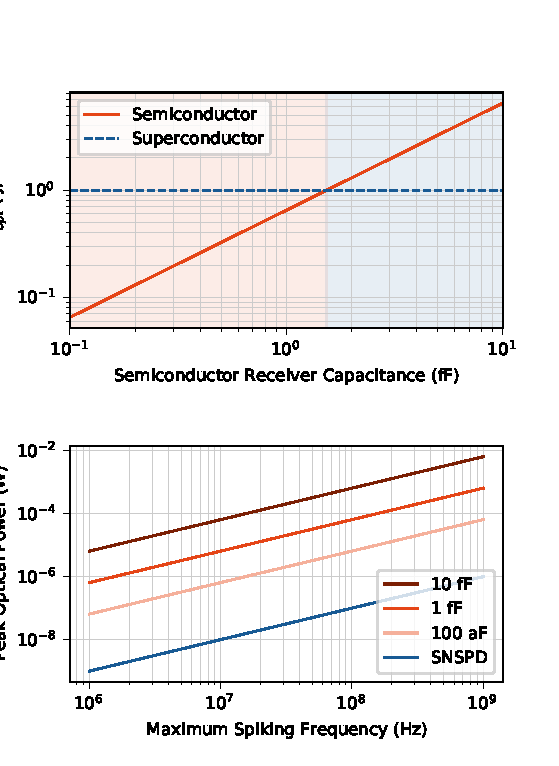
\includegraphics[scale=1]{opticalv2.pdf}
    \caption{A) The minimum optical energy ($\eta = 1$) for an ideal photodiode to generate a 0.8\,V swing is plotted as function of the total receiver capacitance. The optical energy per bit for an SNSPD detector is shown as a dotted blue line. Shaded regions indicate which detector has lower optical energy per \sout{bit} \textcolor{ForestGreen}{synapse event}. B) The required peak optical power to drive 1000 downstream synapses as a function of maximum spiking frequency desired. \textcolor{ForestGreen}{(what are you assuming about the temporal envelope of the light pulse? also, this sub figure (b) isn't explicitly cited in the text. it's a good figure and should be called out)}}
    \label{fig:communication}
\end{figure}

\subsection{Optical Transmitters}
For either superconducting or semiconducting platforms, the transmitter is expected to dominate the power budget of optical links. Transmitters must be waveguide-integrated, capable of delivering sufficient optical power to drive many down-stream synapses, and capable of modulation at speeds greater than the desired maximum spiking frequency of the system. Room-temperature, CMOS-integrated light sources have been a holy-grail in the photonics industry for decades. \textcolor{ForestGreen}{Yet materials integration issues have kept this prized objective out of reach.} The cryogenic environment of superconducting systems significantly improves the prospects for integrated light sources, but comes with its own challenges. Namely, driving light sources with superconducting electronics is \sout{a fundamental challenge} \textcolor{ForestGreen}{difficult due to the low voltages in superconducting circuits}, and will require new interfacing technologies\cite{} \textemdash an obstacle that is completely absent from an all-semiconductor platform.

\subsubsection{Integrated Light Sources}
There are many review articles discussing the long-sought goal of monolithically integrated light sources on silicon substrates \cite{}. Our goal is not to summarize all developments in the field, but to address important factors to consider in choosing a light emitter for this specific application.

The neurons we have envisioned require only incoherent light pulses. Nanolasers are not necessary for this application if nanoLEDs can be constructed with suitable power (see previous section). \textcolor{Violet}{Is that fair? We don't need nanolasers since we don't coherence, but they could be more powerful than LEDs?} \textcolor{red}{yes, you could say something like, ``lasers would be advantageous due to the increased light-production efficiency gained through stimulated emission, but coherence itself is not required.''} NanoLEDs are also attractive for their simplicity of fabrication, lack of threshold current, and improving efficiency with shrinking scale \cite{romeira2019physical}. However, integrating millions of nanoLEDs on 300\,mm wafers (see scaling analysis in section \ref{sec:instantiation}) is still only an aspiration. The difficulty is a fundamental one. \textcolor{red}{(what makes it ``fundamental''?)} Silicon's \sout{excellent} electrical properties\textcolor{ForestGreen}{, low cost, high-quality surfaces, and near-ideal oxide} have resulted in a fabrication ecosystem nearly entirely dedicated to the processing of silicon substrates. Unfortunately, the indirect bandgap of silicon renders it one of the most unpromising semiconductors for light emission. This leaves \sout{only} two \textcolor{ForestGreen}{primary} options: (1) Develop processes to economically integrate direct bandgap materials on silicon substrates at a massive scale or (2) force silicon to emit light through either material and/or environmental modifications. \textcolor{red}{(another option that some may point to is to use off-chip light sources or shared light sources) }

III-V semiconductors are the most commonly used materials for \textcolor{ForestGreen}{light sources used in} optical communication. However, while extensively investigated, integrating III-V materials with silicon still poses significant challenges. A lattice mismatch between most III-V materials and silicon has so far prevented direct epitaxial growth from being a dominant solution.\footnote{Recent developments in this area are encouraging, however. \cite{li2017epitaxial}} Another route to III-V heterogeneous integration involves physically attaching pre-grown III-V crystals onto silicon wafers. A variety of schemes have been proposed, including flip-chip bonding, die-to-wafer bonding, wafer-to-wafer bonding, and transfer printing \cite{zhang2019iii,more,references,jeff,has,a,bunch}. These processes are still unproven at massive scale, and it remains to be seen if they will be an economical solution. \textcolor{red}{(may be worth a tad more discussion of possible light sources for the semiconductor case. what light sources have been demonstrated that produce enough power to serve 1000 connections? how big are they? what is their capacitance? can they be integrated with waveguides? we should cite a few of John Bowers' papers as well as the Ghent/IMEC/LETI papers)}

In contrast, proponents of all-silicon light sources argue that bonding technology will remain expensive and challenging for large-scale integrated photonic circuits. The vision is that the comparatively simple fabrication process for silicon LEDs will enable massive integration density, reminiscent of the success of the homogeneous CMOS process. Main avenues of research include erbium-doped silicon, silicon nanocrystals, strained SiGe, and loop dislocation emitters, among others \cite{pavesi2008silicon,again,more,refs,jeff,has,em}. Additionally, silicon light sources are naturally compatible with silicon waveguides, which potentially reduces coupling losses. However, the performance of silicon light sources has never proven to be competitive with III-V light sources, leading to an unfortunate trade-off between the scalability of silicon and the performance of III-V materials. 

However, for superconducting optoelectronic systems, the cryogenic operation brings significant benefits to light-sources, both silicon and III-V. The efficiency of a light emitter is determined by relative rates of radiative and non-radiative recombination. Upon lowering the temperature from 300\,K to 4\,K, radiative recombination time was demonstrated to decrease by over four orders of magnitude in GaAs/AlGaAs quantum wells, resulting in a corresponding increase in efficiency measured by photoluminescence \cite{gurioli1991temperature}. Even more applicable, the supression of non-radiative recombination paths resulted in 1\%-efficient, waveguide-integrated InP LEDs at 10\,K\textemdash an improvement of two orders of magnitude over room-temperature operation \cite{dolores2017waveguide}. These light sources are already suitable for extremely large neural systems (section \ref{sec:instantiation}) if they can be manufactured at scale. Additionally, spectral broadening from phonon interactions is significantly depressed at low-temperature, making narrow-linewidth emitters more easily achieved. This means that the Purcell Effect\textemdash which increases the radiative emission rate of light emitters coupled to a resonant cavity \cite{}\textemdash is often easier to demonstrate at low temperatures. For silicon light sources, there may be even more benefits in moving to a low-temperature environment. A variety of point defects demonstrate photoluminesence in silicon only at low temperatures, some of which can be patterned and formed easily with ion implantation. In particular, the W-center, an interstitial defect formed through silicon self-implantation has generated significant interest. W-centers have been demonstrated in 300\,mm foundry processes \cite{buckley2020optimization} and have already been integrated with waveguides and SNSPD receivers \cite{buckley2020optimization}. Efficiency is still a major question, however, as the maximum external efficiency reported for a W-center LED is only $10^{-6}$ \cite{bao2007point}, although the internal efficiency may have been significantly higher. \textcolor{ForestGreen}{Point defects have extremely narrow linewidths \cite{}, which indicates potential to leverage Purcell enhancement.}

\subsubsection{Driving Circuitry}
A neuron must be capable of driving a semiconductor light source. The transmitter circuitry is thereby required to produce voltages on the scale of the bandgap of the optical source\textemdash usually on the order of 1\,V. CMOS circuitry, itself a semiconducting technology, naturally operates on this voltage scale rendering the driving circuitry essentially a non-issue. Standard MOSFET LED or modulator driving circuits \cite{oneforleds,oneformodulators} can be straightforwardly adapted for neuromorphic applications. Superconductors, however, operate in an entirely different regime, with signals usually on the order of the superconducting energy gap, which is typically about 1\,mV. The optimal method for interfacing superconducting electronics with semiconductor devices is still an area of active research. Recent progress has been made, however, with devices utilizing the massive change in impedance during the phase transition from the superconducting state to normal metal. In Ref.\,\cite{mccaughan2019superconducting}, a resistive element is heated using 50\,mV pulses to thermally trigger a transition in a superconducting meander. The meander transitioned to a state with resistance in excess of 10\,M$\Omega$ and was used to drive a cryogenic light source. While these results are promising, the light source was only pulsed at only 10\,kHz (due to poor source efficiency) and was fabricated on a separate chip. More work is needed to improve the speed, to monolithically integrate this driving circuitry with LEDs, and to ultimately demonstrate fully functioning optical links using SNSPDs.

\section{\label{sec:soma}Electronic Neuronal Computation}
Electronic circuitry capable of \sout{faithfully emulating} \textcolor{red}{(i don't want people to think we're trying to make devices that follow the Hodgkin-Huxley model)} \textcolor{ForestGreen}{performing neuronal dynamical} operations will also be necessary. While the programability of digital neuromorphic chips will make them a vital tool in the near future, analog circuitry will likely ultimately be more efficient at \sout{simulating} \textcolor{ForestGreen}{achieving} neuronal behavior. Analog CMOS neurons exhibiting complex behavior have been developed over the past few decades. Many of these designs and concepts should be transferable to optoelectronic semiconductor platforms. Additionally, superconducting neural circuits have also been developed and appear capable of implementing \sout{just as sophisticated behavior} \textcolor{ForestGreen}{behavior with the same level of sophistication}. \textcolor{ForestGreen}{Speaking generally, neuromorphic electronic circuits must be capable of achieving synaptic operations such as short-term adaptation \cite{}, long-term potentiation and depression \cite{}, dendritic operations such as thresholding and coincidence detection \cite{}, neuronal threshold adaptation \cite{}, and spike production \cite{}. Here we do not explore details of these operations, but rather address high-level considerations with general applicability to all these neuromorphic operations.}

\subsection{CMOS}
The maturity of CMOS processing has allowed great strides in neuromorphic computing. Digital neuromorphic chips designed for edge applications are nearing commercialization \cite{davies2018loihi, merolla2014million}. While optical communication would likely also be advantageous in digital approaches, we focus on analog CMOS neurons for their perceived efficiency advantages \cite{rajendran2012specifications, mead1990neuromorphic}. Analog CMOS neuromorphic systems have been the subject of intense research since the work of Carver Mead in the late 1980s \cite{1,2}. Mead recognized that many of the behaviors observed in biological cells lent themselves to simple and efficient emulation in analog circuitry \cite{mead1990neuromorphic}. At the most basic level, a neuron must perform three mathematical functions: summation of synaptic functions, temporal filtering, and threshold detection. Summation can be achieved by exploiting Kirchoff's current law. Filtering can be implemented with elementary resistor-capacitor circuits. Thresholding is a natural function of transistors. Building upon this basic mapping, a great variety of analog neurons have been demonstrated to emulate a litany of biologically-inspired neuronal models \cite{indiveri2011neuromorphic,more,more}. It has even been argued that analog neuromorphic circuits are already mature enough to simulate the brain with current technology \cite{hasler2017special}.

However, it must be noted that increasing circuit complexity is usually accompanied by increasing power consumption \textcolor{ForestGreen}{and silicon area}. It was found in the previous section that optical communication requires a minimum of about 1\,fJ of energy to deliver a spiking signal to each synapse. For realistic optical link efficiencies, this value will be at least one or two orders of magnitude larger. Synaptic filtering circuits would therefore ideally operate with an energy budget of 10\,fJ - 100\,fJ \sout{of energy} to process a single spike. For the simplest implementations, synapses may be nothing more than resistive memory element (section \ref{sec:memory}) and a wire. However, more sophisticated synaptic circuits are likely necessary for improved problem-solving ability and greater biological realism \cite{chicca2020recipe}. \textcolor{red}{(description of why short- and long-term plasticity are necessary for cognition/intelligence/learning/adaptation as well as a few references supporting these assertions from neurosci and refs to cmos neuro implementations)} Somatic computation could comfortably consume power larger than that of synaptic processing by a factor of the average fan-out (perhaps 1000). The energy scale of synaptic and neural circuits is set by the value of capacitance used for filtering and the supply voltage ($CV^{2}$). By reducing both the capacitance and voltage, a neuron capable of 25\,kHz spike rates was demonstrated to consume only 4\,fJ/spike \cite{sourikopoulos20174}. Many other analog neurons, with energies ranging from fJ to pJ per spike, fall comfortably below the power consumption of optical communication \cite{indiveri2019importance}. Neurons with maximum spike rates exceeding 100\,MHz have also been demonstrated \cite{schemmel2020accelerated}. Optical communication should face few issues achieving such speeds, if it can be efficiently integrated with these circuits.

Some CMOS neuromorphic circuits have prized bio-realism\textemdash targeting biologically realistic timescales and fan-in. Achieving long time constants commensurate with biology (upwards of 500\,ms) has been achieved using sub-threshold circuits with very low currents \cite{indiveri2011neuromorphic}. These low currents reduce the need for large capacitors that can be difficult to integrate on chip \textcolor{ForestGreen}{due to large area consumption}. In terms of fan-in, most implementations have so far fallen just short of biological levels ($10^3$-$10^4$ synapses per neuron). Fan-in of 256 has been demonstrated for both sub-threshold \cite{qiao2015reconfigurable} and accelerated time circuits \cite{schemmel2020accelerated}. Analyses of specific implementations have suggested that fan-in on the scale of biology is at least theoretically possible \cite{dowrick2018fan, akima2014majority}.  

For a concrete example, a circuit diagram for a memristor implementation of the popular differential-pair integrator (DPI) synapse is shown in Fig. \ref{fig:filtering}(b) \cite{dalgaty2019hybrid}. The DPI produces a decaying exponential waveform in response to an input voltage pulse\textemdash potentially from an optical receiver. This leaky integrator behavior is characterized by a time constant set by the value of the filtering capacitance and the rate of leakage off of the capacitor \cite{chicca2014neuromorphic}. This time constant could potentially even be programmed using memristors\textemdash which is an advantage over superconducting circuits that have been proposed to date. \textcolor{red}{(say a little more about the advantage. what is it? why can't superconductors use this?)}

\begin{table*}[h]
  \begin{center}
    \label{tab:mathtable}
    \begin{tabular}{l|c|r} % <-- Alignments: 1st column left, 2nd middle and 3rd right, with vertical lines in between
      \textbf{Function} & \textbf{Semiconductors} & \textbf{Superconductors}\\
      \hline
      \textit{Summation} & Kirchoff's Law & Mutual Inductors (Faraday's Law)\\
      \textit{Low-Pass Filter} & RC Circuit & LR Circuit\\
      \textit{Thresholding} & Transistors & Josephson Junctions\\
    \end{tabular}
    \caption{Summary of implementations of basic neuronal functions in each platform.}
  \end{center}
\end{table*}

\textcolor{red}{(perhaps we need a sentence or two that says, ``there's tons of literature on cmos neuro, so we don't want to repeat it all. see these review articles. toward the big end (subject of this paper) especially see these articles (spinnaker, brainscales, etc).'')}

\subsection{Superconducting Electronics}
Superconducting neurons have been studied nearly as long as CMOS implementations, with a mapping between neuronal functions and superconducting electronics also identified in the early 1990s \cite{hago1991, hiak1991}. In this case, Lenz's Law, governing the addition of magnetic flux through mutual inductors to superconducting loops provides the necessary synaptic summation function. Filtering is achieved through resistor-inductor blocks.\footnote{Or RC circuits in some cases \cite{crotty2010josephson}.} \sout{Finally,} Josephson Junctions (JJs) provide the requisite nonlinear thresholding element.\footnote{Spiking behavior from superconducting nanowires have also been proposed as an alternative nonlinear element to JJs \cite{toomey2019design}.} A summary of these mappings is given in table \ref{tab:mathtable}. 

Like their CMOS counterparts, many superconducting circuits have now been designed to implement sophisticated neuronal dynamics. Superconducting neuromorphic circuits have been designed to implement a variety of bio-inspired neuron models \cite{crotty2010josephson, toomey2019design, schneider2018tutorial}, sophisticated dendritic processing \cite{shainline2019fluxonic}, and have performed image classification in simulation \cite{schneider2017energy}. Promising concepts for superconducting plasticity circuits and memory are addressed in the next section. The natural spiking behavior of JJs may even require a lower device count than analogous CMOS circuits for various leaky-integrate-and-fire models \cite{crotty2010josephson}. In short, it does not appear that superconducting circuits are any less capable of complex neuronal computation than CMOS platforms.

Superconducting electronics \textcolor{ForestGreen}{has long been pursued for} \sout{is traditionally associated with} gains in energy efficiency and speed. Indeed, superconducting elements dissipate zero static power and spike energies are frequently reported in the sub-fJ range, including refrigeration. This makes it a near certainty that optical communication will dominate power consumption for superconducting optoelectronic systems. In terms of speed, fully electronic superconducting neurons may be capable of spike rates up to 100 GHz \cite{schneider2017energy, schneider2018tutorial}. However, this is orders of magnitude faster than any SNSPD can respond. This marks a notable difference between the superconducting and semiconducting architectures. While optical communication could be integrated with CMOS neurons with no degradation in speed, optoelectronic superconducting systems will likely be significantly slower than their fully electronic counterparts. We believe that this is the cost of highly connected systems. \textcolor{ForestGreen}{However, the extraordinary switching speed of JJs can still be leveraged in optoelectronic networks to perform analog computations within synapses, dendrites, and neurons.}

Somewhat surprisingly, the ability of superconducting electronics to go slow might be just as compelling as their ability to go fast. \textcolor{blue}{Too corny?} \textcolor{red}{No, I like it.} While great effort was needed to implement long, biologically realistic time constants in CMOS neurons, superconducting loops can create essentially arbitrarily long time constants by adjusting \sout{tweaking} the $L/R$ ratio in synaptic and neuronal loops (figure \ref{fig:sup_synapse}). The exact consequences of this capability are unknown, but intriguing, as it has been suggested that the human brain itself is limited by the length of time constants available in its hardware \cite{indiveri2019importance}. The ability to generate dynamics across many orders of magnitude in time also dovetails nicely with suggestions that critical behavior is important for cognition \cite{cocchi2017criticality}. \textcolor{red}{(worth a little more elaboration on this important concept, related to nested frequencies, adaptation across time scales, and power-law memory retention)}

Fan-in has traditionally been considered a liability of superconducting electronics. If this were the case, it would clearly be an impediment to mature superconducting neuromorphic systems. For superconducting neurons designed to use single fluxons as action-potentials, fan-in is still likely to be limited to around 100\cite{schneider2020fan}\textcolor{ForestGreen}{, particularly in situations where a single synapse must be able to drive a neuron above threshold}. However, if signals are allowed to contain multitudes of fluxons \textcolor{ForestGreen}{(analog computation)}, fan-in can likely scale to biological levels through the use of mutual inductors (see Appendix \ref{apx:fan-in}). Using larger signals comes with larger power consumption, but for optoelectronic systems, light production will almost certainly still dominate. This makes the decision to move away from single-flux computing a natural one for superconducting optoelectronic systems, as it solves the fan-in problem with no noticeable increase in power consumption. \textcolor{ForestGreen}{The total system power consumption of large-scale systems remains tractable.}

It is important to recognize that while most diagrams of superconducting circuits (including those here) show many separate biases delivering current to various elements, the ability to construct circuits that can be biased in series will be critical to the scalability of this hardware. A separate bias for every synapse would be absolutely untenable in large-scale systems \cite{sergey}. This mimics the evolution that occurred in superconducting digital electronics, in which the field turned away from the parallel biasing of RSFQ \textcolor{red}{(probably need to define)}, whose current sources dominated the energy budget, and towards the \textcolor{ForestGreen}{current recycling concepts of ERSFQ \cite{}} and serially-biased RQL architecture \cite{tolpygo2016superconductor}. We believe that the neurons designed for the SOENs platform are amenable to serial biasing, but this important point demands further analysis.

A superconducting synaptic filtering circuit is shown in figure \ref{fig:filtering}a. Synaptic weighting is implemented in the receiver circuit (figure \ref{fig:sup_synapse}a), so this circuit block is only responsible for converting a train of fluxons into a decaying exponential \textcolor{ForestGreen}{(post-synaptic potential)} reminiscent of biological and CMOS synapses. A resistor, $r_{si}$ converts a superconducting persistent current loop into a leaky-integrator very similar to the DPI synapse. The time constant is set by $L_{si}/r_{si}$, and the synaptic current can be added to a neuronal circuit through mutual inductors. Unlike the DPI synapse, this circuit does not have a programmable time constant, but does hold the potential to implement a wide range of different time constants by fabricating different values of $L_{si}$ and $r_{si}$. \textcolor{red}{(could it have a programmable time constant if a mosfet or moscap was used? what's the smallest value of resistance one can achieve with a mosfet?)}

\textcolor{red}{(this section could use an additional paragraph getting the reader acquainted with superconducting electronics in general. brief history, latching logic, RSFQ, attempts at digital, C3 program, and reasons for failure. may be a good opportunity to explain why the reasons superconducting digital has failed to displace cmos are not likely to lead to problems in neuromorphic, particularly optoelectronic neuromorphic. i can help write this. please remind me. i've probably already written it somewhere.)}

\begin{figure*}
    \centering
    \includegraphics[scale=.71]{Synaptic Filters.pdf}
    \caption{a) The superconducting synaptic filter receives a train of fluxons. The number of fluxons is proportional to the synaptic weight. $J_{si}$ will convert the fluxon train into a circulating current (whose magnitude is proportional to the number of received fluxons) in the synaptic integration loop, SI. The prescence of $r_{si}$ makes the SI loop a leaky integrator, with time constant $L_{si}/r_{si}$. $I_{si}$ can then be coupled to neuronal integration loop (NI) with mutual inductors. b) A schematic of a differential pair integrator (DPI) synapse featuring memristors \cite{dalgaty2019hybrid}. An input pulse from the optical receiver enables a current proportional to $r_w$ to flow from $C_{si}$ to ground. The rate that $C_{si}$ recharges is determined by $T_3$ and $r_{si}$. This allows synaptic time constants to be programmed. $C_{si}$ and $r_{si}$ form a leaky integrator analogous to superconducting case, and the output current $I_{si}$ can be summed via Kirchoff's Law at a summing node in the somatic circuitry. Plasticity circuits would utilize the various transistors to program values in the memristors.}
    \label{fig:filtering}
\end{figure*}

\section{\label{sec:memory}Synaptic Memory}
It has been apparent to the neuromorphic community for some time that large-scale neural systems will require innovative approaches to synaptic memory. Many modern CMOS neuromorphic systems use bias generators and digital memory to store and control synaptic parameters \cite{liu2014event} Bias generator blocks store parameters digitally and route the appropriate voltages to synaptic and neuronal circuits across the chip. While bias generator circuits are valuable for smaller-scale networks, static power consumption, analog-digital conversion, interconnect charging energy, and inconvenient non-local plasticity updates will make them untenable for larger networks \cite{dalgaty2019hybrid}. These issues have led to a widespread exploration of emerging memory technologies for neuromorphic computing. Extensive investigation is still needed to determine which technology will prove best-suited for large-scale neural systems. However, there are numerous desired characteristics that guide the development of synaptic memories. Among these metrics are weight precision, volatility, area, endurance (the effective number of cycles in a device's lifetime), device-to-device and cycle-to-cycle variability, material compatibility, update symmetry and linearity, write speed, and switching energy. We attempt to provide desired benchmarks for a few of these metrics in the specific case of optoelectronic networks.

\textcolor{ForestGreen}{Because we are considering general cognition rather than acceleration of a specific computation, several comments are in order to expound the motivations for a few important plasticity mechanisms. Across a variety of neural network models, a synapses is specified by an entry in the adjacency matrix specifying the network connectivity and a scalar value specifying the magnitude of the transferred signal. Neural adaptation in many models is through a variation in the threshold. Based on the accumulated knowledge of the neuroscience community, we assume synaptic and neuronal adaptation are more complex than these basic representations.}

\textcolor{ForestGreen}{We assume at least three types of synaptic plasticity are required in large networks accomplishing cognition. Short-term synaptic plasticity on the time scale of an interspike interval during bursting ($\approx$\,10\ms, 100\,Hz) maintains activity within a useful dynamic range and filters noise. Short-term-depressing plasticity acts to limit a runaway post-synaptic response resulting from a high, persistent input signal. Physiologically, this adaptation occurs due to depletion of neurotransmitters on the pre-synaptic cleft. Supply must be synthesized after an episode of bursting. In artificial hardware, other means may be used to play the same role of saturating the synaptic response. Short-term-facilitating plasticity performs the opposite function. A single input spike may not serve to fully activate a synapse, and several input spikes may be required to open the pores that release vesicles containing neurotransmitters. In the presence of noisy communication, when single input synapse events are commonly errant, this mechanism reduces the communication of this noise to the neuron cell body. Many synapses have both of these response characteristics, and their combination can be designed to engineer interesting, frequency-selective transfer functions \cite{}. These short term plasticity mechanisms are useful for stabilizing network activity, filtering noise, and have been shown to aid in the realization of large patterns of correlated activity, an indication of criticality.}

\textcolor{ForestGreen}{Long-term plasticity is typically associated with learning. In the present context we are referring broadly to Hebbian-type activity-dependent plasticity as well as variants such as spike-timing-dependent plasticity (STDP) based on temporal correlations between the two neurons associated with the synapse \cite{}. These adaptations can occur based on single synaptic firing events or can occur much more slowly based on average firing activity. For cognition, we assume principles of hetergeneity are relevant, and desired learning behaviors are achieved through a diversity of adaptive responses of differing magnitudes occurring on a continuum of time scales from the interspike interval to the lifetime of the learning system. It is natural to assume a log distribution of synaptic parameters \cite{}, which brings us to the third form of synaptic plasticity: metaplasticity.}

\textcolor{ForestGreen}{A cognitive system is likely to benefit from incorporating some synapses that adapt rapidly by very large amounts and others that change by small amounts over long time periods. But we also expect networks to benefit from the ability to dynamically adjust the plasticity of different regions at different times. Such metaplasticity provides a chemical signal that modulates the rate and magnitude of STDP updates based on other contextualization from the network. For example, neurons involved in processing vision may benefit if plasticity can be heightened when observing a visually novel scene. While metaplasticity is accomplished in biology through neuromodulators that impact other plasticity mechanisms, in hardware we expect local and regional voltage or current biases that control plasticity to be modulated based on local and regional network activity.}

\textcolor{ForestGreen}{In addition to these synaptic learning/adaptation functions, we assume the firing thresholds of hardware spiking neurons adapt based on network activity. Again we may expect a continuum of magnitude and time-scales, with refraction as a strong, fast negative feedback mechanism, and longer-term threshold adaptation based on a sliding average of firing activity \cite{}. At the synaptic and neuronal circuit levels, we expect cognition to benefit from several adaptive feedback mechanisms implemented across spatial and temporal scales. We refrain from dragging the reader through a discussion of the role of active dendrites in these adaptation mechanisms. Here we consider several of the functional requirements of synaptic learning circuits and their hardware manifestations in both semiconductor and superconductor hardware.}

\subsection{Memory Benchmarks}

\textcolor{blue}{I took out specific references to technologies that you had previously suggested in this subsection. I hope it doesn't make readers jump around too much, but I think it's nice to present the theoretical benchmarks separate from getting lost in the weeds of physical implementations. I saved that for the Proposed Technologies subsection.}
\subsubsection{Endurance}
The large-scale cognitive systems discussed here could be used in at least two different modes. The first is to serially process many separate user-defined tasks over their lifetimes, similar to how modern supercomputers are used. The second is a lifelong learning approach, where the system's weights are allowed to naturally evolve via unsupervised plasticity mechanisms over the course of its operation. In either of these modes, it will be vital that the synaptic weights can be changed throughout the lifetime of the system. This stands in contrast to many edge systems, where inference is a primary (or even sole) mode of operation. Additionally, edge systems will be much less costly to replace, making shorter lifetimes acceptable. Massive neural systems, carrying with them correspondingly sizeable investments \textcolor{blue}{in money and time}, will be desired to have lifetimes on the scale of decades ($10^9$ seconds)\textcolor{blue}{, if not longer}.

The number of times a synapse is updated in its lifetime is a function of neuron spiking frequency ($f$) and the number of synapses that are typically updated after each post-synaptic spike. In neuroscience literature, \textcolor{blue}{evidence has been presented} that the number of active presynaptic inputs required to trigger a postsynaptic spike roughly goes as $\sqrt{N}$, where $N$ is the fan-in of the neuron\textemdash perhaps 1,000 for brain-like systems \cite{vrso1996,vora2005}. \textcolor{blue}{Numerous parameters may be introduced to characterize the synaptic update frequency \cite{fuab2007}. For simplicity, we assume here that all synapses that contributed to the spiking of the post-synaptic neuron} are updated with each spike. \textcolor{blue}{We then estimate} the number of weight updates ($N_{updates}$) in the system's lifetime ($L$) will be:

\begin{equation}
    N_{updates} = \frac{Lf}{\sqrt{N}}
\end{equation}

For a decades-long lifetime, and a mean spiking frequency of 10 kHz, the total number of weight updates will be $10^{11}$. This is a challenging demand for many emerging non-volatile memory technologies (see table \ref{tab:memory_comparison} and section \ref{Proposed}).


\begin{comment}
This is a challenging demand \textcolor{blue}{that far exceeds the endurance of most memristive technologies that rely on the repeated motion of atoms within a host material for electronic property adaptation. Yet even this extreme reliability} has been demonstrated in state-of-the-art memristive and phase change memory (PCM) devices \cite{zhao2020reliability}. \textcolor{blue}{Approaches to memory update that do not require atomic reconfiguration of a material may be better equipped to endure the demands of lifelong learning. In the semiconductor case, this might be accomplished through modification to the voltage on a MOSFET gate, possibly with injection of charge on a floating gate. In the superconductor case, similar functionality can be achieved through modification to the current bias to a JJ, achieved through adaptation of the amount of flux stored in a superconducting loop.}
\end{comment}

\subsubsection{Update Energy}
\textcolor{blue}{Ideally, one would like} the power dedicated to weight updates to be negligible in comparison to the power used for optical communication. Once again invoking the assumption that $\sqrt{N}$ synapses are updated with each postsynaptic spike, we arrive at the following relation between the energy to produce a single spike ($E_{spike}$) and that to update a single weight ($E_{update}$):

\begin{equation}
    E_{update} < \sqrt{N}E_{spike}
\end{equation}

Using the analysis in section 2, roughly 1 fJ of energy needs to be delivered to the receiver in either platform. Assuming a transmitter efficiency of 1\%, this would mean $E_{spike}$ is roughly 100 fJ. Therefore, for a fan-in of 1,000 synapses, $E_{update}$ would ideally be no more than about 3 pJ. Note that this value also includes any energy spent in peripheral circuitry to program the synapse. This suggests that in optoelectronic systems, there is little to be gained by designing update circuits that consume significantly less energy than a few picojoules. This figure appears to be have already been met by several emerging memory technologies \cite{zahoor2020resistive}.

\subsubsection{Update Speed}
While it may tolerable to briefly take synapses offline for weight updates, this is clearly not desired. An ideal system would be capable of implementing synaptic updates within the minimum inner-spike interval. While semiconductor optoelectronic systems can likely produce spike rates in excess of 10 GHz, synapses will need to be taken offline during WRITE operations, as it is highly unlikely that sophisticated plasticity mechanisms can be implemented in under 100 ps. Lower maximum frequencies would allow plasticity to implemented without ever neglecting a spiking event. 100 MHz may be a practical limit for this mode of operation, allowing for 10 ns minimum inter-spike intervals.

\subsection{Weight Precision}
The necessary weight precision will be determined by the specifics of a chosen learning algorithm and the desired application. This has been the subject of much discussion. It has been suggested that 4-bit precision is sufficient for state-of-the-art mixed signal neuromorphic systems \cite{pfeil20124}. Deep learning systems have also demonstrated success with 8-bit precision - a significant reduction from 32-bit floating point numbers \cite{wang2018training}. Hippocampal synapses in rats have been inferred to allow at least 26 different states, which squares nicely with the computer science findings \cite{bartol2015nanoconnectomic}. 

Target values for these key synaptic memory metrics are summarized in Table \ref{tab:memory_metrics}.

\begin{table}[h!]
  \begin{center}
    \label{tab:memory_metrics}
    \begin{tabular}{l|c|r} % <-- Alignments: 1st column left, 2nd middle and 3rd right, with vertical lines in between
      \textbf{Metric} & \textbf{Goal} \\
      \hline
      \textit{Endurance} & $>10^{11}$ updates \\
      \textit{Update Energy} & $<$ 3 pJ\\
      \textit{Update Speed} & $<100$ ns \\
      \textit{Weight Precision} & 4-8 bits
      
    \end{tabular}
    \caption{List of desired performance metrics for synaptic memory in a system with average fan-out of 1000, maximum spike rate of 10 MHz, average spike rate of 10 kHz, and spike energy of 1 fJ.}
  \end{center}
\end{table}

\subsubsection{Programming Signals}
One important criterion that eludes quantitative benchmarking is the complexity of programming circuitry for synaptic memory. Many memory technologies (floating gate, RRAM, and PCM for example) require signals during the programming phase that are significantly different (either in strength or duration) from the signals produced in the normal operation of the network. This often requires extra circuitry that reads the local network activity and decides when to take the memory device offline to apply a WRITE operation with these tailored programming signals. This peripheral circuitry can sometimes be significantly different from that used for the rest of the hardware. We are not claiming that such a scheme is untenable for any inherent reason, but only that it is important to include the complexity of programming circuitry when comparing memory technologies. Superconducting loop memory (discussed in section \ref{Loops}) is particularly intriguing from this standpoint, as the plasticity circuits operate with  nearly identical signals and circuit blocks as those found in the rest of the network.

\subsection{Proposed Technologies}\label{Proposed}
\subsubsection{Room-temperature Technologies}

Many technologies have been proposed to implement synaptic weighting for room-temperature neuromorphic hardware, each with strengths and weaknesses \cite{upadhyay2019emerging}. The quest to find a suitable device for local synaptic memory dates back to the origins of the field, when Carver Mead and colleagues were investigating floating gate transistors \cite{diorio1998floating}. Since then, floating gate synapses have been used to implement STDP \cite{ramakrishnan2011floating} and are attractive as a mature alternative to emerging devices. However, there are concerns about high programming voltages, speed, and endurance that have made researchers turn to other technologies \cite{zahoor2020resistive}. \textcolor{blue}{Because modification of the charge on a floating gate requires significantly different voltage levels and signal times than the spiking signals transmitted from neurons to synapses, this otherwise ideal memory mechanism has not led to large-scale learning systems. Memristive devices \cite{stsn2008,yast2012,ab2018}, commonly used in resistive random-access memory (RRAM)} have emerged as a \textcolor{blue}{popular} alternative, with recent demonstrations including monolithic integration with CMOS \cite{yin2019monolithically} and unsupervised pattern recognition with a simple network of synapses \cite{ielmini2018brain}. However, questions remain about high variability (both cycle-to-cycle and device-to-device) \cite{dalgaty2019hybrid}, endurance, linearity, and the number of internal states \cite{zahoor2020resistive}. Phase Change Memory (PCM) is another intriguing option, with its own demonstration of STDP \cite{ambrogio2016unsupervised}, and is more mature than RRAM. Thermal management and energy consumption have been raised as issues \cite{upadhyay2019emerging, zahoor2020resistive}. Ferroelectric transistors present another interesting alternative, but likely require new material development. Spin-torque memory, 2D materials, and organic electronics have also been proposed as solutions. Interested readers should consult one of the many review articles on this topic \cite{kim2018recent, upadhyay2019emerging, zhang2020brain}. In short, the field is burgeoning with new devices for synaptic memory, but to-date none has been dominant enough to monopolize the \textcolor{blue}{research field.} Lastly, we include a table, adapted from \cite{zahoor2020resistive} that compares a few promising technologies and compares them to the goals we laid out for large-scale optoelectronic networks. While there is still significant progress needed to make these memory, the benchmarks for large-scale optoelectronic systems seem to be within the realm of possibility for both RRAM and PCM.

\begin{table}[h!]
  \begin{center}
    \label{tab:memory_comparison}
    \begin{tabular}{l|c|c|r} % <-- Alignments: 1st column left, 2nd middle and 3rd right, with vertical lines in between
      \textbf{Metric} & \textbf{Floating Gate} & \textbf{RRAM} &\textbf{PCM} \\
      \hline
      \textit{Endurance} & $10^{5}$ & $10^{6}-10^{12}$* & $10^{9}$  \\
      \textit{Update Energy} & \textbf{$\textbf{10}$ fJ} & $\textbf{.1}$ \textbf{pJ} & $10$ pJ\\
      \textit{Update Speed} & $10$ $\mu$s  & $\textbf{10}$ \textbf{ns} & $\textbf{50}$ \textbf{ns}\\
    \end{tabular}
    \caption{Comparison of the current state of three leading technologies for synaptic memory. Metrics that have already met the conditions laid out in table \ref{tab:memory_metrics} are in bold. *The high endurance RRAM measurement was achieved in a binary mode.}
  \end{center}
\end{table}

\subsubsection{Superconducting Technologies}
Many of the aforementioned technologies may also be operational at cryogenic temperatures for use in superconducting optoelectronic systems, but little work has been done in this regard. Instead, two other types of memory, only accessible at low temperatures, have received the most attention: Magnetic Josephson Junctions (MJJs) and superconducting loop memories. MJJs are extremely low-energy, non-volatile, two-terminal devices that are functionally analogous to room-temperature memristive devices. Superconducting loop memories, on the other hand, are close analogues of floating gate transistors (with circulating current playing the role of trapped charge), but operate on different principles than any of the other memories mentioned.

\subsubsection{Magnetic Josepson junctions}
\textcolor{blue}{A Josephson junction (JJ) is formed from two superconducting electrodes separated by a tunneling barrier.} If a ferromagnetic material is placed within the \textcolor{blue}{tunneling barrier}, either in the form of nanoclusters or continuous films, the critical current of the junction can be controlled by changing the alignment of magnetic moments within the insulator. The magnetic order of the ferromagnetic materials can be programmed with current pulses in the presence of an external magnetic field, providing an analog, nonvolatile memory. For cryogenic \textcolor{blue}{applications}, volatility takes on a slightly new meaning. For a memory to be nonvolatile in this context, it must preserve its state upon both the removal of electrical power and upon warming up to room temperature. \textcolor{blue}{MJJs are nonvolatile with respect to removal of electrical power and can retain their state upon heating to around 200\,K. Further stability up to 300\,K remains the subject of research.} 

MJJs provide remarkable synaptic performance \textcolor{blue}{with respect to the metrics given in Table \ref{tab:memory_metrics}}. The synaptic update programming is on the order of femtojoules (\textcolor{blue}{after multiplying by $10^3$ to account for cryogenic cooling}), commensurate with firing rates exceeding 100\,GHz, and can be fabricated at the scale of tens of nanometers. \textcolor{blue}{A tradeoff occurs between the size of the MJJ and the number of analog levels of magnetization, as smaller junctions contain fewer nanoscale magnetic clusters that can be reoriented. Regardless, even for relatively large junctions with many analog levels, the size of  MJJs is inconsequential compared to the size of other components of superconducting synapses, such as mutual inductors used in coupling between synapses and the neuron cell body.} \textcolor{red}{(will this comment make sense? is it necessary to give a rough overview of the synapses and neurons under consideration at the beginning of the document?)} All of these metrics \textcolor{blue}{surpass the requirements} for optoelectronic networks, and can be exploited in all-electronic superconducting networks as well. More work is needed to analyze the scaling potential of MJJs \textcolor{blue}{with respect to yield}. The magnetic fields used during programming can be produced with magnetic control lines, but spin-torque mechanisms may provide a more scalable solution. Peripheral circuitry involved in applying programming pulses and \textcolor{blue}{endurance with respect to repeated realignment of the magnetic moments merit further investigation} \cite{schneider2018ultralow}. \textcolor{blue}{While the energy, speed, area, and weight precision, meet the requirements specified in Table \ref{tab:memory_metrics}, the ability to modify the state of the MJJ using the same signals as are sent from neurons to synapses remains a technical challenge and potential barrier to straightforward implementation of large-scale, unsupervised learning. These challenges are analogous to the challenges faced by memristors and phase-change memory elements, wherein current or voltage pulses are required in addition to those being produced by neurons for signaling to synapses.}

\subsubsection{Loop Memory}\label{Loops}
Superconducting loop memories \textcolor{blue}{have been in use for decades by the superconducting electronics community \cite{vatu1998,ka1999}, but are not ideal for large memory arrays commonly utilized as RAM in digital computing due to the large size as compared to semiconductor alternatives. In the case of optoelectronic spiking neural systems considered here, the objective is not to produce large RAM arrays, and size as well as addressing challenges do not emerge as significant impediments. Therefore, straightforward extensions of binary loop memories} are the synaptic memory technology \textcolor{blue}{that appears most promising} for the SOENs platform \cite{sh2018,shainline2019superconducting}. In these memory cells, circulating current persists indefinitely in a loop of superconducting wire. The current in the loop can be controlled by adding/removing fluxons (the quantized units of magnetic flux) with standard JJ circuitry. This memory loop is then inductively coupled to a wire supplying a bias current to a Josephson Junction at the synapse ($J_{sf}$ in figure \ref{fig:sup_synapse}). Each time the SNSPD detects a photon, the biased junction will add an integer number of fluxons to another integrating superconductive loop (analogous to the membrane capacitance of a neuron). The number of fluxons added to the integration loop is a function of the bias supplied to the JJ, which is determined by the magnitude of current circulating in the memory loop. \textcolor{blue}{The number of analog memory levels in the loop is determined by the inductance of the loop, which is easily set with the length of a wire. High-kinetic-inductance materials \cite{} enable memory storage loops with over a thousand levels (10 bits) to be fabricated in an area of 5\,\textmu m $\times$ 5\,\textmu m (check).}

This approach has several advantages. The memory is nearly analog and updates are nearly linear. Memory is updated by the switching of a JJ, which involves only a change of the phase of the superconducting wave function. While most memristive devices require physical changes to the material (ion transport, filament formation, crystallization, etc.) which can lead to degradation and limited endurance, there appear to be no limit to the number of times that loop memory can be updated. Loop memory is also attractive from a fabrication perspective as it requires no additional materials. Further, the simplicity of the memory lends itself favorably to 3D integration. Plasticity circuits based on loop memories will also operate at the energy scale of single photons and flux quanta ($\sim 10^{-19}$\,J) which is commensurate with the rest of the circuitry in the network. This allows weight updates to be performed with the spikes the network produces in standard operation, cutting down significantly on peripheral circuitry. There is no need to engineer differently shaped pulses for READ and WRITE operations, and the synapse does not need to be taken offline during programming. Simulations have demonstrated STDP learning with circuits containing only four additional Josephson Junctions \cite{shainline2019superconducting}. 

Still, \textcolor{blue}{two aspects of} loop memory are concerning. First, \textcolor{blue}{memory represented by current circulating in a loop persists as long as superconductivity is maintained, even without applying any power source. However, as soon as superconductivity is broken (by raising the temperature of the system, for example), the memory is lost. The temperature of the system may need to be raised to perform maintenance or inadvertently if the system power supply fails.} If this memory is to be preserved during a warmup of the network, it must be first transferred to some other memory storage system. \textcolor{blue}{An exciting prospect is for memories gained through unsupervised plasticity during normal network activity to be transferred to a less volatile storage mechanism such as MJJs, perhaps during a type of sleep phase. But a mechanism for this memory transfer remains to be discovered. The second weakness of loop memory is the size.} The employed superconducting loops, \textcolor{blue}{as well as the transformers that couple them}, will be large compared to all of the other solutions discussed. \textit{Size estimate depends on if we're using SNSPDs or fluxons.} However, \textcolor{blue}{the consequences of these large-area components must be considered in the context of the entire system, which we discuss in Sec.\,\ref{sec:instantiation}.} 

%this is not incompatible with the size of superconducting receivers which are already on the order of $1000 \mu m^2$ and the area concerns are mitigated by the excellent potential of loop neurons for 3D integration.

\section{\label{sec:instantiation}Physical Instantiation}
\textcolor{ForestGreen}{Here we attempt to anticipate requirements for the physical realization of optoelectronic spiking neural systems comprising 10 billion to 100 billion neurons with 100 trillion synapses. We begin this analysis with purely mathematical considerations from graph theory, which inform us as to how many synaptic connections are required to maintain a given average path length across the network. This consideration appears central to efficient communication and information integration in spiking neural systems, is likely the primary reason the brain prioritizes extensive communication infrastructure, and provides a hardware-agnostic foundation on which we base the subsequent spatial analysis.}

\textcolor{ForestGreen}{From graph theory metrics, we proceed to general spatial considerations. Moving from abstract mathematics to a physical instantiation, we make several specifying assumptions: 1) optoelectronic circuits will be fabricated on the two-dimensional surfaces of wafers using the sequential, layered processing techniques that have enabled VLSI circuits; 2) the wafers have a diameter of 300\,mm; 3) multi-wafer systems are constructed by stacking multiple wafers in columns and assembling these columns into three-dimensional architectures; 4) free-space optical communication can be used to signal from a wafer to the two wafers directly adjacent in the vertical direction; 5) inter-wafer couplers are available between each wafer and the four wafers that reside in the same plane in the cardinal directions; and 6) all other communication across the network occurs over optical fibers that fill space between the wafers. With such a construction in mind, the analogy between the grey and white matter in the brain is apparent: the grey matter comprising the computational circuits consists of the hardware integrated on the wafers, while the white matter comprising the communication infrastructure consists of tracts of fiber optic cables spanning the network. Illustrations to clarify the concept are shown below.}

\textcolor{ForestGreen}{With a specific hardware concept specified, we turn attention to considerations pertinent to the fabrication of the wafer-integrated circuits. The photonic and electronic circuits that must be realized have been described above in Secs. \ref{sec:soma}, \ref{sec:communication}, and \ref{sec:memory}. Here the primary considerations relate to the integration of photonic with electronic components and the benefits of dense multi-planar integration. We consider specific processing challenges that appear inevitable for multi-planar realization of semiconductor circuits, superconductor circuits, or photonic components. Challenges are present in all cases, but the challenges differ based on the technology.}

\textcolor{ForestGreen}{With a specific construction concept in mind, and having analyzed optoelectronic integration at the wafer scale, we proceed to estimate the connectivity, volume, power consumption, and cooling requirements of a brain-scale spiking neural system realized in this form. We return to metrics from graph theory to assess whether the necessary connectivity can be retained across the network hierarchy. We estimate the total spatial extent of a system, accounting for grey and white matter, as well as the number of 300-mm wafers necessary for the construction, and we determine that it is likely to be possible to cool such systems using water for semiconductors or helium for superconductors.}

\subsection{Considerations from graph theory}
\textcolor{ForestGreen}{Neuron in brain regions active in cognition, such as the cerebral cortex and hippocampus, are characterized by a high degree of connectivity\textemdash often in excess of ten thousand connections per neuron \cite{brsc1998,bu2006}. These connections often extend across appreciable spatial distances. Creating and maintaining these connections comes with high metabolic and spatial costs. The severely constrained biological brain would not support these expenditures if they were not supremely advantageous to cognition \cite{busp2012}.}

\textcolor{ForestGreen}{One reason why such high connectivity is advantageous relates to efficient communication across the network. Cognition in spiking neural systems is supported by bursts of activity in which neuronal assemblies temporarily coordinate their firing activity. The fastest such oscillations in the cerebral cortex and hippocampus occur at roughly 80\,Hz (gamma oscillations \cite{bu2006}), and it appears crucial that neurons are capable of activating one another within a small number of periods of these oscillations to rapidly respond to changes in stimulus or internal network activity. This rapid communication can only be achieved if the average path length across the network is small. In the language of graph theory, a network is a collection of nodes connected by edges. To calculate the shortest average path length across the network, one calculates the number of edges that must be traversed to travel from each node to every other node in the network. One takes the mean of this quantity over all pairs of nodes in the network. The shortest average path length ($\bar{L}$) is a simple, global metric that offers a glimpse at the efficiency with which information can be communicated across the network.}

\begin{figure}
    \centering
    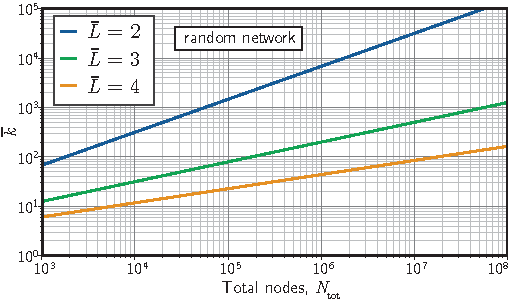
\includegraphics[width=8.6cm]{degree__vs__num_nodes.pdf} % random_graph__connections_vs_num_nodes
    \caption{Average node degree required to maintain a certain network path length as a function of the number of nodes in the network.}
    \label{fig:degree_vs_num_nodes}
\end{figure}
\textcolor{ForestGreen}{By considering the relationship of $\bar{L}$ to the number of nodes and edges in a graph, we can gain insight into the number of synapses required to efficiently interconnect a given number of neurons in artificial cognitive hardware. In a random network, nearby and distant connections are equally probable. The average path length across such networks achieves a lower limit for a given number of edges connecting a given number of nodes. By considering the average number of edges (synaptic connections, $\bar{k}$) required to achieve a given average path length in a random network as a function of the number of nodes in the network (neurons, $N_{\mathrm{tot}}$), we can estimate a lower limit on the number of synapses that each neuron must have for efficient communication. The number of edges required to achieve an average path length $\bar{L}$ across an Erd\"{o}s-R\'{e}nyi random graph with $N_{\mathrm{tot}}$ nodes can be obtained analytically as \cite{frfr2004}}
%\begin{equation}
%\bar{L} = \frac{\mathrm{ln}(N_{\mathrm{tot}}-\gamma)}{\mathrm{ln}(\bar{k})} + \frac{1}{2},
%\end{equation}
\begin{equation}
\label{eq:degree}
\bar{k} = \mathrm{exp} \left[ \frac{\mathrm{ln}(N_{\mathrm{tot}})-\gamma}{\bar{L}-1/2} \right],
\end{equation}
where $\gamma \approx 0.5772$ is Euler's constant. This relationship is plotted in Fig.\,\ref{fig:degree_vs_num_nodes} for several values of $\bar{L}$. For a randomly connected network with $10^6$ neurons, each neuron must make nearly 10,000 connections to support an average path length of two, and 200 synapses must be formed to support a path length of three. For a network with $10^8$ neurons, more than 100,000 synapses are required for a path length of two, and more than 1,000 for a path length of three. The human hippocampus is a module with roughly $10^8$ neurons, each with 10,000-50,000 nearly spatially random connections. The objective of achieving an average path length between two and three may be an important reason why the hippocampus prioritizes this exceptional degree of connectivity. The cerebral cortex in the human brain contains more than $10^{10}$ neurons, each with roughly 10,000 connections. This analysis indicates that a path length between two and three cannot be achieved across the entire cortex, and accordingly this vast organ of cognition is constructed with a hierarchical, modular architecture \cite{si1962,ne2006} with high connectivity and efficient communication within smaller modules, and more sparse connectivity between modules separated by larger distances \cite{mo1997,mela2009,bosp2015,beba2017}.

\textcolor{ForestGreen}{While more sophisticated graph metrics can further elucidate the network concepts underlying cognition \cite{busp2009,sp2010}, the simple, global metric of average shortest path length can help inform scaling analysis of artificial cognitive hardware. We next consider the constraints $\bar{L}$ puts on the size of synaptic circuits.}

\subsection{Generic spatial constraints}
\label{sec:spatial_constraints}
\textcolor{ForestGreen}{Based on the significance of the interplay between the hippocampus and cerebral cortex in cognition \cite{frbu2016}, we assume hardware for artificial neural systems will make use of similar architectural principles. However, artificial hardware does not have the functionality of bottom-up nanofabrication, as employed by biological neural systems. Here we assume optoelectronic circuits will be fabricated using the conventional sequential, planar processing techniques of the silicon microelectronics industry. We further specify to consideration of 300-mm wafers and seek a relationship between the network path length and the size of components on the wafer.}

The area of a neuron occupied by its photonic waveguides can be approximated in a similar manner to the wires for electronic circuts \cite{ke1982}. This gives the following expression for the area of passive photonic circuitry:
\begin{equation}
\label{eq:area_p}
A_p = \left( \frac{k w_{wg}}{p_p} \right)^2
\end{equation}
$p_p$ is the number of photonic waveguide planes, $k$ is the degree of each neuron (assumed identical), and $w_{wg}$ is the pitch of waveguides. The area of a neuron due to electronic circuits is given by
\begin{equation}
\label{eq:area_e}
A_e = \frac{k w_{sy}^2}{p_e}
\end{equation}
$w_{sy}$ is the width of a synapse and $p_e$ is the number of planes of electronic circuits. Both of these areas are subject to the constraint that
\begin{equation}
\label{eq:area_x}
A_x N_{300} = A_{300}.
\end{equation}
From these relations and Eq.\,\ref{eq:degree} we can estimate the maximum average shortest path length as a function of the width of a synapse [Fig.\,\ref{fig:path_length__vs__width}(a)] or the width of a waveguide pitch [Fig.\,\ref{fig:path_length__vs__width}(b)]. 
\begin{figure}
    \centering
    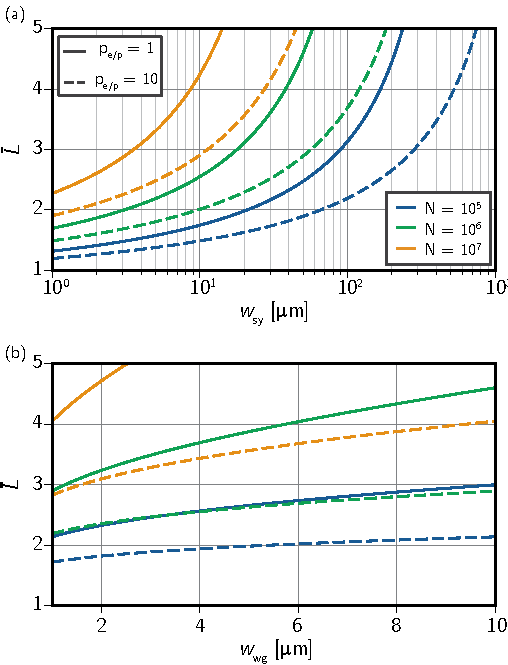
\includegraphics[width=8.6cm]{path_length__vs__width.pdf}
    \caption{Path length vs width.}
    \label{fig:path_length__vs__width}
\end{figure}
A key message of these plots is that it will be very difficult to integrate ten million neurons on a wafer while maintaining a short path length near 2.5. Even if only one million neurons per wafer are sought, multiple planes of active electronic circuits and passive photonic waveguides will make a significant difference in connectivity as quantified through network path length.

While Figs.\,\ref{fig:path_length__vs__width} only considers one or 10 planes, Fig.\,\ref{fig:num_planes} shows the number of planes required to achieve a path length of 2.5 as a function of the number of neurons on the wafer for several values of synapse and waveguide size. We will refer to Figs.\,\ref{fig:path_length__vs__width} and \ref{fig:num_planes} to guide the reasoning presented in the subsequent discussion of fabrication.
\begin{figure}
    \centering
    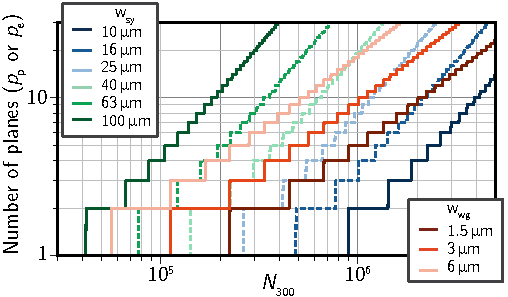
\includegraphics[width=8.6cm]{num_planes.pdf} 
    \caption{Num planes.}
    \label{fig:num_planes}
\end{figure}

%\begin{figure}
%    \centering
%    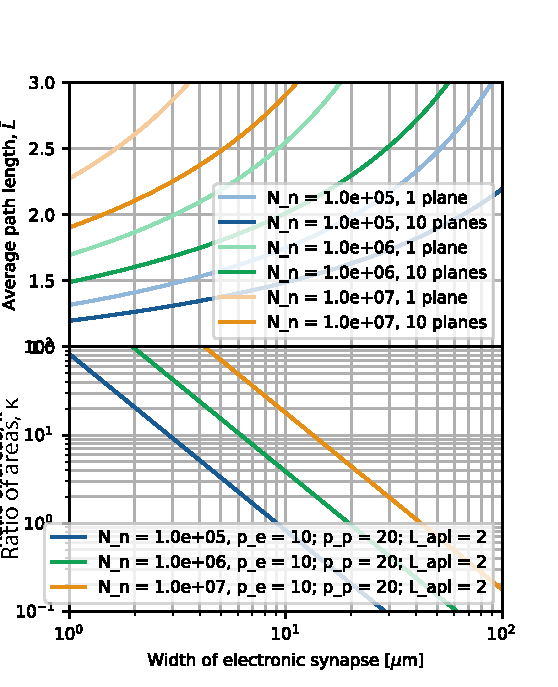
\includegraphics[width=8.6cm]{area_scaling.pdf}
%    \caption{Area scaling.}
%    \label{fig:area_scaling}
%\end{figure}

\subsection{Wafer fabrication and processing}
\label{sec:fabrication}
At the time of this writing, the CMOS industry is the height of information technology. Future hardware for AI may use entirely different manufacturing techniques, but any such revolutionary technology (i.e., leveraging bottom-up nanofabrication) requires sufficient technological evolution as to be essentially unpredictable at this point as well as at least several decades from being able to achieve optoelectronic neural systems. As with the spatial considerations above, we restrict our attention to optoelectronic hardware fabricated with the tools and techniques brought to their present state of maturity by the silicon microelectronics industry.

We briefly summarize and specify the processing we envision. A 300-mm silicon wafer is the primary vessel for all subsequent fabrication. MOSFETs may be in bulk silicon, SOI, or deposited poly-crystalline silicon. Dopants defining nMOS and pMOS transistors are formed with photolithography, ion implantation, and rapid thermal annealing up to the range of 1000\,\textcelsius for dopant activation. Insulators SiO$_2$ and SiN$_x$ are deposited between electric layers using chemical vapor deposition, not necessarily at elevated temperature. Passive wiring layers are formed from sputtered metals, and vias are realized by etching through insulators, backfilling with metals, and removal of excess material through planarization. In a process with many wiring layers, as we envision here, most process steps are followed by planarization through chemical-mechanical polishing, leaving a SiO$_2$ or SiN$_x$ surface with less than 0.5\,nm root-mean-square roughness present for each subsequent layer. Superconducting wiring can be fabricated in the same manner, with niobium instead of copper or aluminum, as used in CMOS. Metal contacts on silicon are formed with interfacial silicides and contact annealing around 600\,\textcelsius, while most superconducting wires are niobium or a niobium alloy, and no annealing is required with contacting the leads of JJs; we assume JJs are Nb/AlO$_x$/Nb superconductor-insulator-superconductor junctions with external shunt resistors. No annealing is required to establish contacts between Nb and the PdAu shunt resistors or to make contact with high-kinetic-inductance wiring layers, typically comprised of NbTiN, MoSi, or other amorphous or polycrystalline superconductors, which can also be sputtered at room temperature. The same insulating materials deposited through chemical vapor deposition are expected to be used in the superconducting process. These insulating dielectrics are expected to be used for photonic waveguides as well, with light being guided in materials such as deposited amorphous silicon (a-Si) or SiN$_x$ clad with lower-index SiO$_2$. Inter-photonic-layer coupling can be accomplished either evanescently \cite{} or through integrated vertical mirror pairs \cite{}.

With these basic fabrication concepts in mind, we proceed to consider specific aspects of the relevant components. 

\subsubsection{Electronic circuits}
We are considering the feasibility of constructing cognitive systems with $10^{10}$ neurons and $10^{14}$ synapses. Nowhere near this scale of system will fit on a single wafer. If $10^5$ neurons are on a wafer, the same number of wafers will need to comprise the system assembly. It would be more convenient if there were orders of magnitude more neurons per wafer than wafers in the assembly.

MOSFETs are the most impactful information technology in human history. Silicon is the material of choice for this technology because it is cheap due to ubiquity in the earth's crust, is conducive to making MOSFETs due to the excellent native (and engineered) oxides, can be purified and refined into large crystalline boules which can then be cut into large wafers, and these wafers have favorable mechanical and thermal properties for processing and system integration. These features as well as advances in photolithography are related process equipment have supported the good run of exponential scaling \cite{} that has provided the physical foundation for the present age of information. In the context of integrated silicon microelectronic circuits, scaling refers to the simultaneous adjustment of multiple spatial features defining MOSFETs, capacitors, and wires while maintaining similar operating voltages \cite{Keyes}. Much of the improvement in computing technology since the 1960s is traced to these relatively simple spatial considerations. 

Given the evident benefits of integrating larger numbers of MOSFETs in smaller space, one might expect the devices to be realized in 3D volumes rather than on 2D surfaces. Along these lines, An important message of Sec.\,\ref{sec:spatial_constraints} is that multiple active SCPs are necessary if we aim to integrate $10^6$ neurons on a wafer, which would mean there were one-hundred times fewer wafers in the assembly than neurons on the wafer. From Fig.\,\ref{fig:area_scaling} we see that 10 SCPs are required to achieve a path length between two and three if all the electronic activity for each synapse fits within an area 10\,\textmu m $\times$ 10\,\textmu m. As described in Sec.\,\ref{sec:memory}, many of the synapses with complex plasticity mechanisms adapting on short and long time scales make use of MOSFETs in the subthreshold operating domain for analog signal processing. Many of these circuit demonstrations have occupied areas much larger than this 10\,\textmu m $\times$ 10\,\textmu m target. However, many also used older CMOS technology nodes with larger feature sizes. Subthreshold MOSFETs are more straightforward to realize with lower device variability if feature sizes are bigger, although modern nodes do offer potential \cite{}. Still, synapse circuits are much more complex than a single transistor and benefit from sizeable capacitors for integration and filtering. It is not clear further CMOS scaling will compactify synaptic circuits to the point where they are smaller than the photonic axons, and it is clear that optoelectronic hardware for cognition will benefit from such multiplanar integration.

The most straightforward route to integrating multiple planes of MOSFETs would be to utilize multiple deposited planes of semiconductor with insulators and vias between. Indeed, this approach has been pursued for transistors based on polysilicon, primarily for memory applications. Direct, monolithic integration of multiple planes of polysilicon mosfets has not become the industry standard for several reasons. First, for digital processors or applications where high-performance transistors are desired, polysilicon is not optimal. Subthreshold, analog operations are likely to prefer crystalline silicon for transistors. It is not impossible to construct multiple planes of crystalline silicon, but it is usually accomplished through wafer bonding, which adds significant cost relative to deposition. Second, MOSFETs depend on accurate placement of dopants and junctions for operation. These fine features are achieved with photolithography, ion implantation, and rapid-thermal annealing for dopant activation. Once formed, further high-temperature processing causes dopant diffusion, which has deleterious effects on MOSFET performance. But polysilicon is typically deposited at high temperatures, so after a single plane of MOSFETs has been fabricated, repeating the procedures of polysilicon deposition, implantation, and annealing is difficult to accomplish without degrading the underlying layers. Third, the metal wires used to make contact to silicon and to interconnect transistors are based on Al and Cu, which cannot be processed above 600\,\textcelsius. Aluminum is commonly used to make contact to transistor gates, and this material melts at 660\,\textcelsius. Yet polysilicon is usually deposited near 900\,\textcelsius, so one cannot form interconnects between planes of MOSFETs without significant process modifications. 

We see that a single plane of MOSFETs requires high temperature processing for dopant activation and metal contacts that must be fabricated subsequently. These processing constraints have limited the ability of the community to achieve sequential, monolithic integration of multiple planes of MOSFETs. Instead, the drive for dense volume integration has led to the development of die stacking \cite{} and wafer bonding \cite{} processing techniques. With these processing techniques, entire integrated circuits with MOSFETs, resistors, capacitors, and interconnecting wires are fabricated, and then two or more such systems are interfaced through bonding techniques that can be utilized at the die or wafer scale. Fully processed die can be integrated at the package level, often making use of an interposer chip, but for the large-scale cognitive computing applications under consideration, the most extreme forms of large-scale integration are required. Achieving complex synaptic circuits that fit within 100\,\textmu m $\times$ 100\,\textmu m is a challenge, yet from Fig.\,\ref{fig:xx} we see that for a module of $10^6$ neurons to fit on a 300-mm wafer, all synaptic response and adaptation circuits must fit within 30um x 30um to achieve an average path length of 2.5, even if 10 planes of active circuits are employed. To achieve a brain-scale system, $10^4$ such units must be assembled. Approaching this challenge with die-level processing and die-level 3D integration appears laborious. Achieving $10^6$ neurons on a wafer with a single active plane of electronics will require that all synaptic functions be achieved with 10um x 10um\textemdash not an unimaginable feat, but several orders of magnitude smaller than state-of-the-art. \textcolor{red}{(is that correct? still must check several other references)}

To reach the scale of integration under consideration with CMOS electronics, several research frontiers should be explored. First, functional synaptic plasticity circuits with adaptation mechanisms across temporal scales must be implemented with as compact a footprint as possible. Adaptive materials may play a role, but trading size or simplicity for functionality is likely to degrade cognition. Making use of recent technology nodes may help \cite{}, and new memory devices may also play a key role. A great strength of CMOS is the compact footprint, and that must be leveraged if brain-scale cognition is the objective. Second, due to the evident challenges with 3D MOSFET integration, wafer-scale heterogeneous 3D integration becomes important for this specific information processing application. At present, this approach to system fabrication involves thinning the silicon handle wafers of upper layers, etching holes through the substrate, and filling with metal to form through-silicon-vias. The wafers are thinned to reduce parasitic resistance and capacitance. This process is currently expensive and time-consuming with sub-optimal yield, but further progress is likely. In the present context, the use of optical through-silicon vias may prove enabling. We revisit this concept in Sec.\,\ref{sec:yy}. \textcolor{red}{(need calculation of TSV energy consumption vs capacitance vs optical energy consumption, also size comparison)}

How difficult is the situation with superconducting electronics? Figures .. are agnostic to the mechanisms of the electronic circuits, so integrating a million neurons on a wafer while maintaining a network path length of 2.5 still requires all synaptic circuits fit within 10um x 10um or that multiple planes of adaptive electronics can be utilized. In the superconducting case, the active components are JJs and the passives are inductors and transformers. JJs will never be as small as MOSFETs \cite{tolpygo2016superconductor}, but the area of synaptic circuits is not limited by JJs. Large inductors or transformers that couple flux from storage loops to receiving SQUIDs are likely to be the components that consume the most area. The sizes of these components is determined by the critical current of the junctions used in the SQUIDs ($I_c$) and the permeability of free space ($\mu_0$). From the considerations given in Appendix \ref{apx:squid_size}, we find $w_{\mathrm{sq}} \approx \mu_0/E_{\mathrm{sq}}$, where $w_{\mathrm{sq}}$ is the width of the SQUID, and $E_{\mathrm{sq}}$ is the energy required for the SQUID to produce a pair of fluxons\textemdash the elementary operation of a SQUID. For superconducting synapses, there is a clear size-energy trade-off. Both quantities are related to the junction critical current. Figure .. shows the approximate SQUID width and energy per fluxon pair as a function of the junction $I_c$. We find that a SQUID has a width of 10\,\textmu m if $I_c = 60$\,\textmu A. With this $I_c$, xx fluxons can be produced in analog processing of each synapse event before consuming the same energy as is required to produce the 10 photons for neuron-to-synapse communication, assuming a light-source efficiency of yy. If $I_c = 100$\,\textmu A is chosen, $w_{\mathrm{sq}} = $ ..\,\textmu m, and fluxonic and photonic energy consumption are matched if xx fluxons are produced per synaptic firing event.
\begin{figure}
    \centering
    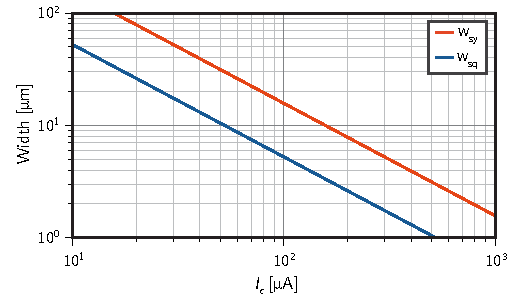
\includegraphics[width=8.6cm]{squid_size.pdf}
    \caption{Squid size.}
    \label{fig:squid_size}
\end{figure}

A superconducting synapse with complex functionality is likely to be more complex than a single squid, likely incorporating multiple SQUIDs coupled via inductive flux-storage loops and transformers. Assuming a spatial equivalent of four SQUIDs are involved in a synapse (2 x 2 array), and leaving additional space for wiring and to avoid cross talk, consider the case where the synapse width $w_{\mathrm{sy}} = 3w_{\mathrm{sq}}$. In Fig. .. we see that 20\,\textmu m $\le$ $w_{\mathrm{sy}}$ $\le$ 30\,\textmu m can be achieve with 50\,\textmu A $\le$ $I_c$ $\le$ 80\,\textmu A. This $I_c$ range achieves a reasonable size/energy balance and is suitable for low noise operation and being driven by SPD currents. It is also worth noting that SQUIDs cannot be packed arbitrarily densely, as cross talk between transformer input coils and flux-shielding wires will limit how closely SQUIDs can be packed. The trends of Fig. .. will be difficult to maintain beyond $I_c = 100$\,\textmu m. From Fig. .. we see that $10^6$ neurons can be incorporated on a 300-mm wafer with $w_{\mathrm{sy}} = 25$\,\textmu m, provided eight circuit planes are utilized. As in the semiconductor case, we see the significance of wafer-scale processing of multiple SCPs.

Fabrication of complete superconducting electronic circuits can be accomplished with temperatures never exceeding 180\,\textcelsius. Integrated circuits with two stacked planes of JJs have been demonstrated by two research laboratories \cite{}. Two stacked planes of SNSPDs have been demonstrated by a third group \cite{}. The most sensitive aspect of a JJ is the tunneling barrier, which is about 3nm thick in the junctions likely to be employed for this purpose. These tunneling barriers appear able to endure the requisite processing of subsequent layers and can be fabricated on surfaces of other sputtered materials or planarized layers with tolerable degradation. Because junction $I_c$ depends exponentially on the tunneling barrier thickness, cross-wafer uniformity is paramount. The ability of mature foundry processes to realize low spatial variation across the wafer, and the ability of neural circuits to tolerate such variability are open questions.

To reach the scale of integration under consideration with superconducting electronics, several research frontiers should be explored. First, several features of superconductor processing appear advantageous for platform scalability, but the potential for further 3D integration of active superconducting layers merits significant future research. Because the sizes of JJ circuits cannot be scaled down with a Moore's-Law-type effect, the potential for wafer-scale 3D integration should be pursued immediately. Second, experimental demonstrations of synaptic plasticity functions are required to bolster confidence that this approach to neuromorphic circuits may be competetive with CMOS from an information-processing perspective, and these demonstrations should be carried out in densely packed circuits, as flux trapping and cross talk are important considerations that may have deleterious effects at the system level. 

Some readers may take a different message from Fig. .., arguing instead that 3D integration is not necessary as it is trivial to make synapses smaller than 10\,\textmu m $\times$ 10\,\textmu m, as a single memristor, floating-gate MOSFET, or phase-change material of size 100\,nm $\times$ 100\,nm performs adequate synaptic functions. While the work in these areas represent impressive scientific progress, the neuromorphic functionalities of artificial synapses based on a single material or device are often far less sophisticated than the adaptation mechanisms of synapses in the brain.  Achieving conceptually similar functionalities may require complex integrated circuits. The full suite of adaptation mechanisms discussed in Sec.\,\ref{sec:memory} has never been demonstrated simultaneously in a single synaptic circuit, let alone every synapse in a large system. This is not a criticism of work in the field, but rather recognition of the difficulty of the task and the sophistication of biological hardware. When considering the potential for artificial technologies to achieve the performance of the brain, we must assume dynamical mechanisms of synapses that neuroscience has revealed to be of consequence do indeed impact the system's ability to achieve cognition.

Still, it is important to note that even if $p_p = p_e = 1$, it is still possible to fabricate wafers with $10^6$ neurons, provided $\bar{k} = 100$, giving $\bar{L} = 3.5$. While this does not match the short path lengths of cognitive circuits in the brain, such a network is likely to have significant technological and scientific utility while offering an intermediate-term practical objective.

\subsubsection{Passive photonic circuits}
From Figs. .. we see that to maintain a path length between two and three on a 300-mm wafer with $10^6$ neurons, roughly six waveguide planes (three ACPs) are required. Here we assume these planes are simple, passive photonic waveguides fabricated using the same materials and techniques as the dielectric insulators used in CMOS electronics. Such planes of routing waveguides are analogous to wiring layers in an electronics process and are generally straightforward and inexpensive to fabricate, with relatively large feature sizes due to the wavelength of light under consideration. Multiple planes of these dielectric waveguides are comprised of amorphous silicon (aSi), silicon nitride (SiN$_x$) and silicon oxynitride (SiO$_x$N$_y$), and such multiplanar waveguides have been fabricated by numerous research groups \cite{}. These ``back-end'' photonics process modules are becoming commonplace in commercial photonic foundries, such as AIM and IMEC \cite{}. 

In these photonic waveguide structures, light is confined by the index contrast between the higher-index waveguide material and the lower-index cladding. The index of aSi can be as high as 3.5, that of SiN near 2, and that of SiO$_2$ 1.45. SiO$_2$ is typically used for the cladding, and essentially continuous gradation of index values between 1.45 and 3.5 can be achieved by adjusting the composition of SiO$_x$N$_y$. With a higher index contrast, light is more tightly confined in the waveguide, so waveguide widths and bending radii can be reduced. However, scattering loss due to roughness of the waveguide sidewall increases as the index contrast squared \cite{} ($\Delta n^2$). Like the SQUID, this introduces a size-energy trade-off. Based on the considerations given in Appendix \ref{apx:wg_size}, we expect $w_{\mathrm{wg}} \sim \lambda_0/\sqrt{E_{\mathrm{wg}}}$, where $w_{\mathrm{wg}}$ is the width of a waveguide, and $E_{\mathrm{wg}}$ is the energy lost to scattering during transit. 

One has a fair amount of control over the operating point in width-propagation-loss space. Due to the $\Delta n^2$ dependence of the attenuation length, a small change in index contrast can deliver an appreciable benefit in propagation loss. Similarly, a small increase in waveguide width can significantly reduce the field intensity on the waveguide sidewalls and further reduce scattering loss. It is reasonable to expect that higher-index waveguides will be used for dense local connectivity, with gradually lower-index being used in subsequent layers for longer-distance connections. From Fig. .. we see that densely packed waveguides of 1.5\,\textmu m pitch could achieve a path length of 2.5 across a network of $10^6$ neurons on a 300-mm wafer with about three paris of waveguide planes, while wider 3\,\textmu m waveguides will require about four pairs of planes, and 6\,\textmu m would require 10 pairs of planes. Perhaps two ACPs of 1.5\,\textmu m-pitch aSi waveguides could be used for local routing, two ACPs of lower-index SiN waveguides for intermediate range, and 6\,\textmu m-wide SiN or SiON for long-haul, cross-wafer communication. Low-temperature-deposited SiN has already demonstrated adequate performance \cite{}.

While the materials and processing steps used for dielectric waveguides are the same as those for insulators in electronics processes, the waveguide layers are generally thicker. The waveguides themselves are typically 100\,nm - 300\,nm, and two planes of waveguides must be separated by about a wavelength ($\approx 1$\,\textmu m) to avoid cross talk or scattering loss, whereas a copper wire is typically about 100\,nm and an insulator between two metals is also about 100\,nm. One new consideration that is thus introduced is the strain of these waveguide and spacer films, which can lead to wafer bow and possibly delamination. A film of 10x thickness brings 10x the strain. It may be necessary to compensate the typical compressive stress of SiO$_2$ films with tensile stress in the electronics layers or in SiN waveguides. For example, sputter deposition conditions can adjust the strain of Nb wiring layers to be either compressive or tensile with little degradation of $T_c$.

This consideration of waveguide size and loss is related to the ability to achieve communication across the system. Network analysis across multiple contexts reveals that efficient communication is often achieved through connectivity obeying Rent's rule \cite{}, which observes that the number of connections emanating from a network partition containing $n$ nodes follows a power law of the form
\begin{equation}
\label{eq:rent}
e\propto n^\gamma,
\end{equation} 
where $0 \le \gamma \le 1$. Gradually larger partitions are often interpreted as representing higher levels of information-processing hierarchy \cite{}, so $\gamma < 1$ indicates gradually diminished connectivity up the cognitive hierarchy, with $\gamma = 1$ indicating that each node has equivalent connectivity on all scales of hierarchy. This scaling can be quantified in terms of a topological dimension, $D_T = 1/(1-\gamma)$. In biological neural systems, a topological dimension between three and four is discovered \cite{}, indicating the exceptional connectivity across spatial scales effectively increases the dimension of the space in which the network is embedded. We are therefore guided to seek interconnection technology with $\gamma \approx 0.8$, which requires many long-distance connections. However, this value is appreciably less than unity, so there need be fewer long-distance connections relative to the number of local connections. Thus, the fact that long-distance waveguides must be slightly wider can be accommodated while maintaining a topological dimension greater than three. Given a specified topological dimension, photonic loss budget, and number of ACPs, one can judiciously engineer the dielectric composition of each waveguide layer. 

The systems under consideration do not terminate at the wafer's edge. To achieve brain-scale cognition, we expect communication to extend between wafers over fiber-optic waveguides. Optical fibers can be coupled to on-chip or on-wafer photonic waveguides through evanescent coupling \cite{} or mode-matching with grating couplers \cite{}. Whereas the wafer-integrated waveguides we have been discussing are 6\,\textmu m or smaller, a fiber-optic waveguide is a cylinder 125\,\textmu m in diameter. The index contrast is very low (xx \%), so the propagation losses are extremely low (yy dB/m). This low loss enables communication across large systems at the speed of light, but presents a challenge in maintaining the Rentian scaling of Eq.\,\ref{eq:rent} beyond partitions containing one or a few wafer modules. We consider this concept further in Sec.\,\ref{sec:...} related to realizing large systems.

To reach the scale of integration under consideration with passive photonic waveguides, several research frontiers should be explored. First, wafer-scale integration of multiple planes of low-loss waveguides of varying indices of refraction must be demonstrated for routing across spatial scales. Second, the stress of these films must be controlled or compensated to enable scaling to the order of 10 planes without incurring wafer bow that impedes further processing. Third, further work on high-yield, low-loss fiber-to-wafeguide couplers is required to show that the requisite level of inter-wafer connectivity can be achieved. Forth, theoretical analysis of full-connectivity achieving Rentian scaling while constrained by propagation loss and spatial limitations could reveal additional limits on the applicability of photonic interconnectivity for large-scale cognitive systems.

\subsubsection{Detector integration}
For the artificial neural systems under consideration, detectors and light sources bridge optical and electrical activity, but while the system requires only one light source per neuron, it requires one detector at each synapse. This consideration inclines us to seek methods for integrating photodetectors with every ACP.

In the semiconductor case we consider photodiodes (PDs) comprised of reverse-biased $p-i-n$ junctions either adjacent to or as the body of an integrated waveguide \cite{}, and for the superconductor case we consider superconducting-nanowire single-photon detectors (SPDs) created on top of photonic waveguides and evanescently coupled to the optical mode \cite{}. A semiconductor material with absorption at the wavelength of communication (1\,\textmu m $\le \lambda \le$ 1.6\,\textmu m) must be integrated with passive photonic waveguides. Waveguide-integrated detectors are commonly realized with SiGe or simply Ge for high performance \cite{}, and can also be made from polysilicon for increased manufacturability \cite{}. In terms of speed, these detectors have far better performance than required for the present application, reaching up to 45\,GHz \cite{}. As shown in Fig.\,.., it is unlikely to realize light sources with sufficient output intensity to drive synaptic detectors this fast. From a materials integration perspective, both SiGe and polySi are reasonable candidates and have been demonstrated with capacitance on the order of 1\,fF\textemdash as required for the receiverless concept described in Sec.\,\ref{sec:communication}. The detectors can be as small as 4\,\textmu m in length while maintaining sufficient absorption and fabricated with a maximum temperature of 660\,\textcelsius \cite{}. The leakage current in the SiGe detectors of Ref.\,\cite{} was relatively high at x nA when reverse-biased at y V, but lower speed and responsivity may be acceptable, so leakage current may be reduced. The leakage current of x pA in the polySi photodetectors of Ref.\,\cite{} under 10 V reverse bias is likely tolerable for the present application, as -10\,V is not necessary here. The detectors of Ref.\,\cite{} were manufactured in a bulk CMOS electronics process, fully integrated with MOSFET control circuits. In that work, the same polysilicon layer used for transistors was used for waveguides and detectors. From an area perspective, it will be advantageous if they can be on separate planes.

On the superconducting side, waveguide-integrated superconducting-nanowire single-photon detectors (SPDs) are a relatively straightforward technology. SPDs are thin films (3\,nm - 10\,nm) of superconducting wires deposited through sputtering, commonly at room temperature, and patterned into wires from 50\,nm to 5\,\textmu m wide using conventional lithography and etching. Common SPD materials include polycrystalline NbTiN and amorphous WSi and MoSi. These films can be deposited on many substrates, and functioning on top of an insulator with 0.5\,nm roughness, such as SiO$_2$ or SiN after planarization, does not appear to appreciably degrade performance. Two overlapping planes of SPDs have been demonstrated with multiple materials \cite{}. Many groups have demonstrated waveguide-integrated SPDs with multiple waveguide and SPD materials \cite{}. WSi SPDs have been waveguide-coupled to III-V and Si integrated light sources. Multiplanar integration of room-temperature-deposited passive photonic waveguides and evanescently coupled SPDs appears quite promising for the present application.

An SPD operates under current bias, and the current is directed to another circuit branch when a photon is detected (see Fig.\,\ref{fig:sup_synapse}). As mentioned in Sec.\,\ref{sec:xx}, it is imperative that superconducting circuits be biased in series to avoid requiring impractical current supplies. In one sense, SPDs are promising for this mode of operation, as large numbers can be fabricated with similar critical current and detection plateau \cite{buta2020}. However, the material with the best detection plateau (WSi) is also a material with a $T_c$ that is slightly too low, requiring operation around 2\,K rather than the desired 4.2\,K of liquid helium. Improvements with detection plateau in NbTiN and MoSi are forthcoming \cite{}, and the associated materials challenges do no appear insurmountable.
 
To reach the scale of integration under consideration with waveguide-integrated detectors, several research frontiers should be explored. Primarily, for semiconductors it will be a worthwhile endeavor to integrate multiple planes SiGe or polySi detectors atop MOSFETs performing synaptic computations interconnected with passive routing waveguides. For superconductors, these detectors must be monolithically integrated with JJ synaptic circuits. Subsequent 3D integration should follow. This work is necessary to demonstrate the scalability necessary to achieve billions of synapses on a 300-mm wafer. On the superconductor side, materials improvements to enable many SPDs with similar detection plateaus to be biased in series are necessary if a billion synapses are to operate simultaneously on a wafer without formidable wiring challenges. 

\subsubsection{Light source fabrication}
We require one light source per neuron. More may be advantageous but are not assumed in the present construction. The hardware burden is thus reduced by three orders of magnitude relative to synapses. We expect a single plane of light sources to suffice, and they with their driver circuitry need not be miniscule. If a 300-mm wafer contains $10^6$ neurons, each can occupy and area 250\,\textmu m $\times$ 250\,\textmu m. Light sources filling this area must produce xx J pulses for semiconductor synaptic detectors and yy J pulses for superconductor detectors, and for both cases light sources of this size producing this power output have been demonstrated \cite{}. Area is not the primary constraint. We are limited by integration.

Consider semiconductors. If a light source as simple as a transistor could be easily integrated with CMOS, computing hardware would be transformed, and there would be no need to make the case for optoelectronic neural systems. All large-scale computing systems would be optoelectronic. Realization of this integration has proved elusive. The indirect band gap of silicon ensures that straightforward optical emission between the band edges is inefficient at room temperature, and still a slow and likely useless process at low temperature. Many attempts to overcome this limitation have been made \cite{shxu2007}, including: quantum-confined structures such as Si/Ge supperlatices and Si nanocrystals \cite{}; point-defect \cite{} and extended-defect emitters \cite{}; engineering of the local density of optical states to enhance emission rates \cite{}; and hexagonal silicon, curiously grown on GaAs \cite{}. While several of these approaches have resulted in LEDs with reasonable output power around 1\,mW \cite{}, none have satisfied the requirements of integration with CMOS while providing sufficient optical power for the primary objective of digital communication. Even if the goal is to transmit optical signals from one source to one detector, digital communication requires bright light sources so that bits represented by roughly 1000 photons can be received within 100\,ps or less for 10\,Gbps or faster data rates. Such a feat requires only 1\,\textmu W of continuous-wave output power. Alas, many in the field have stopped holding their breath. To our knowledge, no viable light source of any material has been monolithically integrated with CMOS electronics and used in a functional optoelectronic circuit. \textcolor{red}{(have we missed this in our reading of the literature? seems like we would know about it, but it also seems like at least something janky must have been demonstrated)}

For many applications, utilization of III-V laser diodes fabricated independently and coupled to a silicon photonic or optoelectronic chip via fiber has proven sufficient and cost effective. Compound-semiconductor laser diodes based on vertical cavities or edge emission perform well for digital communication in telecommunications applications that span the globe, within data centers to connect server racks, within heterogeneous packages, and even on chip for processor-to-memory communication \cite{}. However, for the present application where a million light sources are required per wafer and ten-thousand wafers are envisioned in an assembly, monolithic integration would be supremely advantageous, if not squarely essential. 

The promise of optoelectronic integration of III-V light sources with silicon electronic circuits has loomed large for decades \cite{}, and many have not settled for a package-level approach to optoelectronic integration \cite{}. The core of III-V/Si integration results from the lattice mismatch between Si (xx\,nm) and GaAs (yy\,nm) or its alloys. Direct growth of GaAs on Si results in defect-ridden material with poor optical and electronic properties. Many solutions have been and continue to be explored. A thick buffer of GaAs can be grown in Si to take up the strain of the lattice mismatch before growing the quantum-confined III-V gain medium \cite{}. This approach has the drawback that the thick buffer makes electronic integration between the underlying Si transistors and the upper light-source layers difficult to realize. It is also not clear that the CMOS can endure the temperatures required for III-V growth. 

If the III-V gain medium is comprised of quantum dots, higher density of strain-related defects can be tolerated, as these crystal imperfections are less likely to strike a zero-dimensional quantum dot than a plane of quantum wells, and a defect that incapacitates a quantum dots removes one of many dipole emitters from the ensemble, rather than introducing a non-radiative recombination pathway that shunts carriers from a wide region of a quantum well. 

Still, the challenges associated with quantum dots grown on CMOS have led many to pursue heterogeneous integration techniques involving substrate transfer of processed III-V devices to processed Si wafers \cite{}. Such transfers can take place at the device, die, or wafer scales. For the present application, 300-mm wafer integration would be most desirable, but III-V wafers are difficult to scale with high quality above 200\,mm. Wafer scaling is challenged by the fact that the substrate crystal has two different atoms per unit cell, leading to significantly higher defect density relative to Si. The growth chambers used to produce quantum heterostructures for electrical injection into quantum dot arrays typically process these smaller wafers, and it is unclear (to the authors) how practical it will be to scale this infrastructure to 300-mm. 

If the wafer sizes cannot be made to match, patches of optical gain material will need to be transferred to the Si handles. This can be accomplished through bonding techniques or transfer printing. The processing steps necessary to form the optical structures and their electronic contacts may be performed before or after the III-V material has been transferred to the CMOS wafer. Research into light-source integration on Si has been active for decades, and no clear convergence to a single most promising approach is evident.

Due to the thermal processing requirements of CMOS, the light sources will almost surely be fabricated last, at the top of the stack. However the light-emission medium is integrated with the rest of the network, electrical contact will need to be made to the driving circuitry, and optical coupling will need to be established to the passive photonic waveguides. The parasitics at electrical contacts are likely to increase with coarser scales of heterogeneous integration, and evanescent coupling between optimized laser structures and passive silicon photonics infrastructure tends to result in pesky inefficiencies. Nevertheless, these details are not likely to be deal breakers. The severe challenge is achieving the requisite scale of integration.

If one wished to leverage III-V light sources with superconducting electronics, many considerations are similar. One would still be inclined to base the fabrication on a large silicon wafer, even if nary a transistor is employed. The silicon handle provides a good mechanical platform, and thermally oxidized Si is an ideal surface to deposit the first superconducting layer of a process. However, in contrast to the semiconductor case, light sources are likely to go down first in a superconducting optoelectronic process. Again, the reasons are thermal. Whether for wafer bonding or metallization of contacts, the optical gain structures are likely to require temperatures of perhaps up to 600\,\textcelsius. It appears more straightforward to perform these steps to realize the cores of the transmitters before depositing an insulator, establishing vias, planarizing, and beginning the superconducting and passive photonic modules. These modules need not exceed 200\,\textcelsius, so the light sources are likely to survive subsequent processing unscathed. Schematics of the semiconducting and superconducting processes are shown in Fig.\,\ref{fig:fabrication_stack}.
\begin{figure}
    \centering
    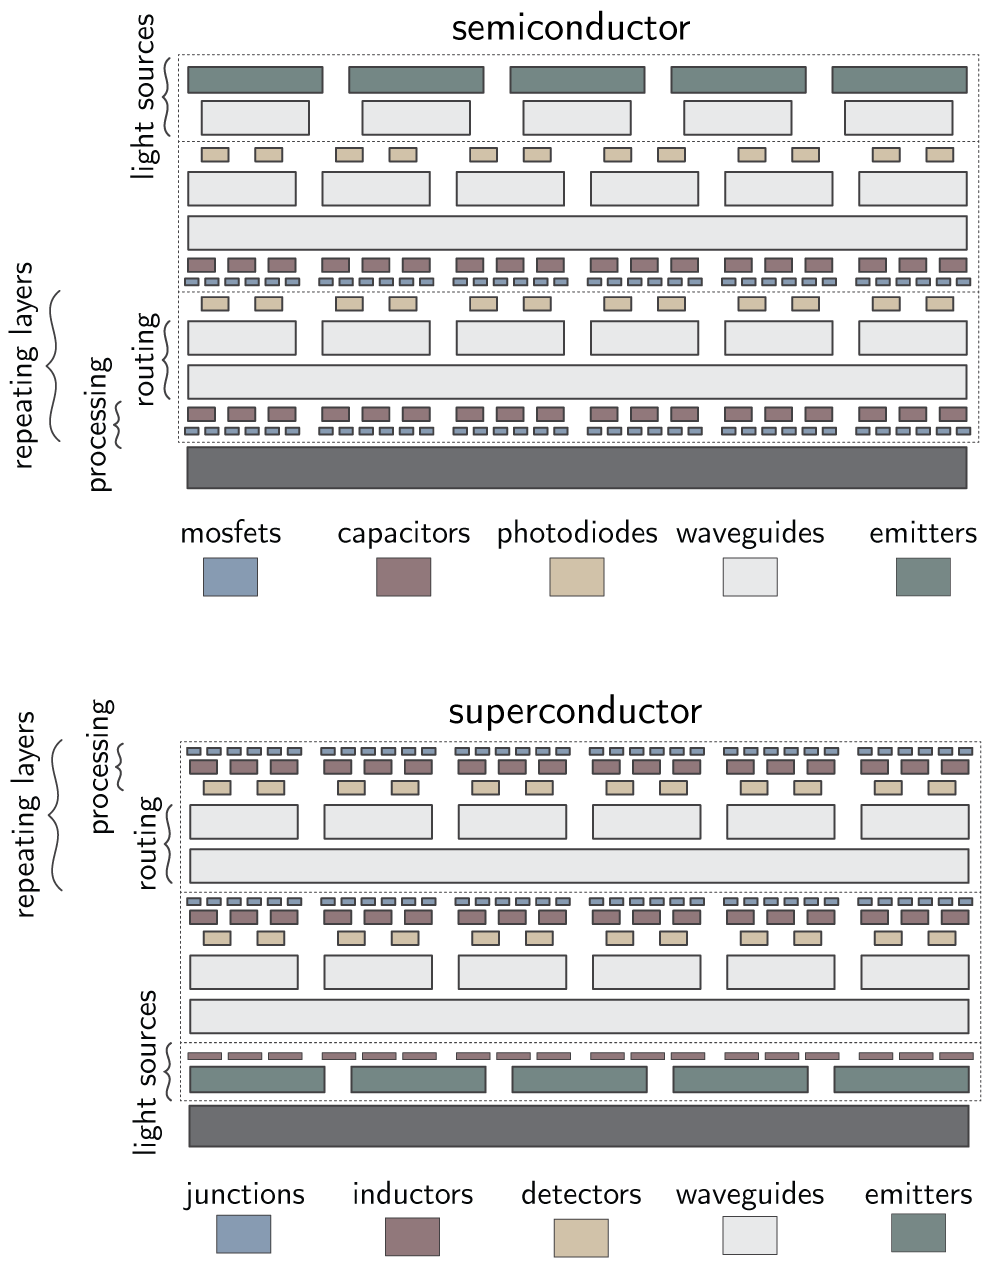
\includegraphics[width=8.6cm]{fabrication_stack.png}
    \caption{Fabrication stack. (a) Semiconductor. (b) Superconductor.}
    \label{fig:fabrication_stack}
\end{figure}
We emphasize that...

For both the semiconducting and superconducting cases, only a single plane of emitters is likely to be required per wafer. The paths toward light source integration that have been trodden have been rocky, and the climb ahead thus described appears steep. Yet the requirement of only one plane is merciful. At present, perhaps the most concrete statement we can make is that large-scale integration of III-V light sources with semiconducting or superconducting electronics is far from certain. 

Some of the strongest arguments for superconducting electronics in large neural systems come from the light-source ramifications. Let us consider three key features that emerge when systems are designed to operate at low temperature alongside superconductors. First, at low temperature, all light sources improve significantly (Sec.\,\ref{fig:communication}), but silicon light sources improve to the point where they may be viable for this application. Second, superconducting detectors dramatically reduce to output requirements of the light sources by three orders of magnitude. Third, cognitive computing with spiking neurons appreciably relaxes the speed demands relative to digital communication. Light sources improve while demands are relaxed. 

To reach the scale of integration under consideration with integrated light sources, several research frontiers should be explored. On the semiconductor side, wafer-scale optoelectronic integration is crucial. This comes as news to no one. On the superconductor side, the question of whether silicon light sources will suffice must be answered urgently. If this is determined affirmative, the consequences appear significant. If even this cannot be accomplished with the great chasm of that infamous indirect gap, full attention should be directed to integration of superconducting electronic circuits atop compound semiconductor light emitters.

\textcolor{red}{(somewhere might want to quickly make the case that shared light sources are problematic, as is wdm)}

\subsubsection{Wafer-scale processing}
We respect that the reader is weary, so here we quickly acknowledge that the optoelectronic integration challenges described here in Sec.\,\ref{sec:fabrication} are not the only class of fabrication challenges to emerge in this context. Digital processors fit on a die, and a thousand die across a wafer are processed identically, using exactly the same reticle set. In the present context, cross-wafer \textit{heterogeneity} is necessary. Attention must be paid to efficient use of reticles when realizing wafer-scale patterns so the cost of masks does not become prohibitive. The hierarchical, modular construction of the network \cite{} must be efficiently captured in the mask set.

%the nature of superconductivity is that the quality of devices is not as affected by material crystallinity, so lower temp processing is adequate, thus enabling 3D integration

\subsection{Constructing large systems}

Large systems may bear some resemblance to the sketches in Fig.\,\ref{fig:system}.
\begin{figure*}
    \centering
    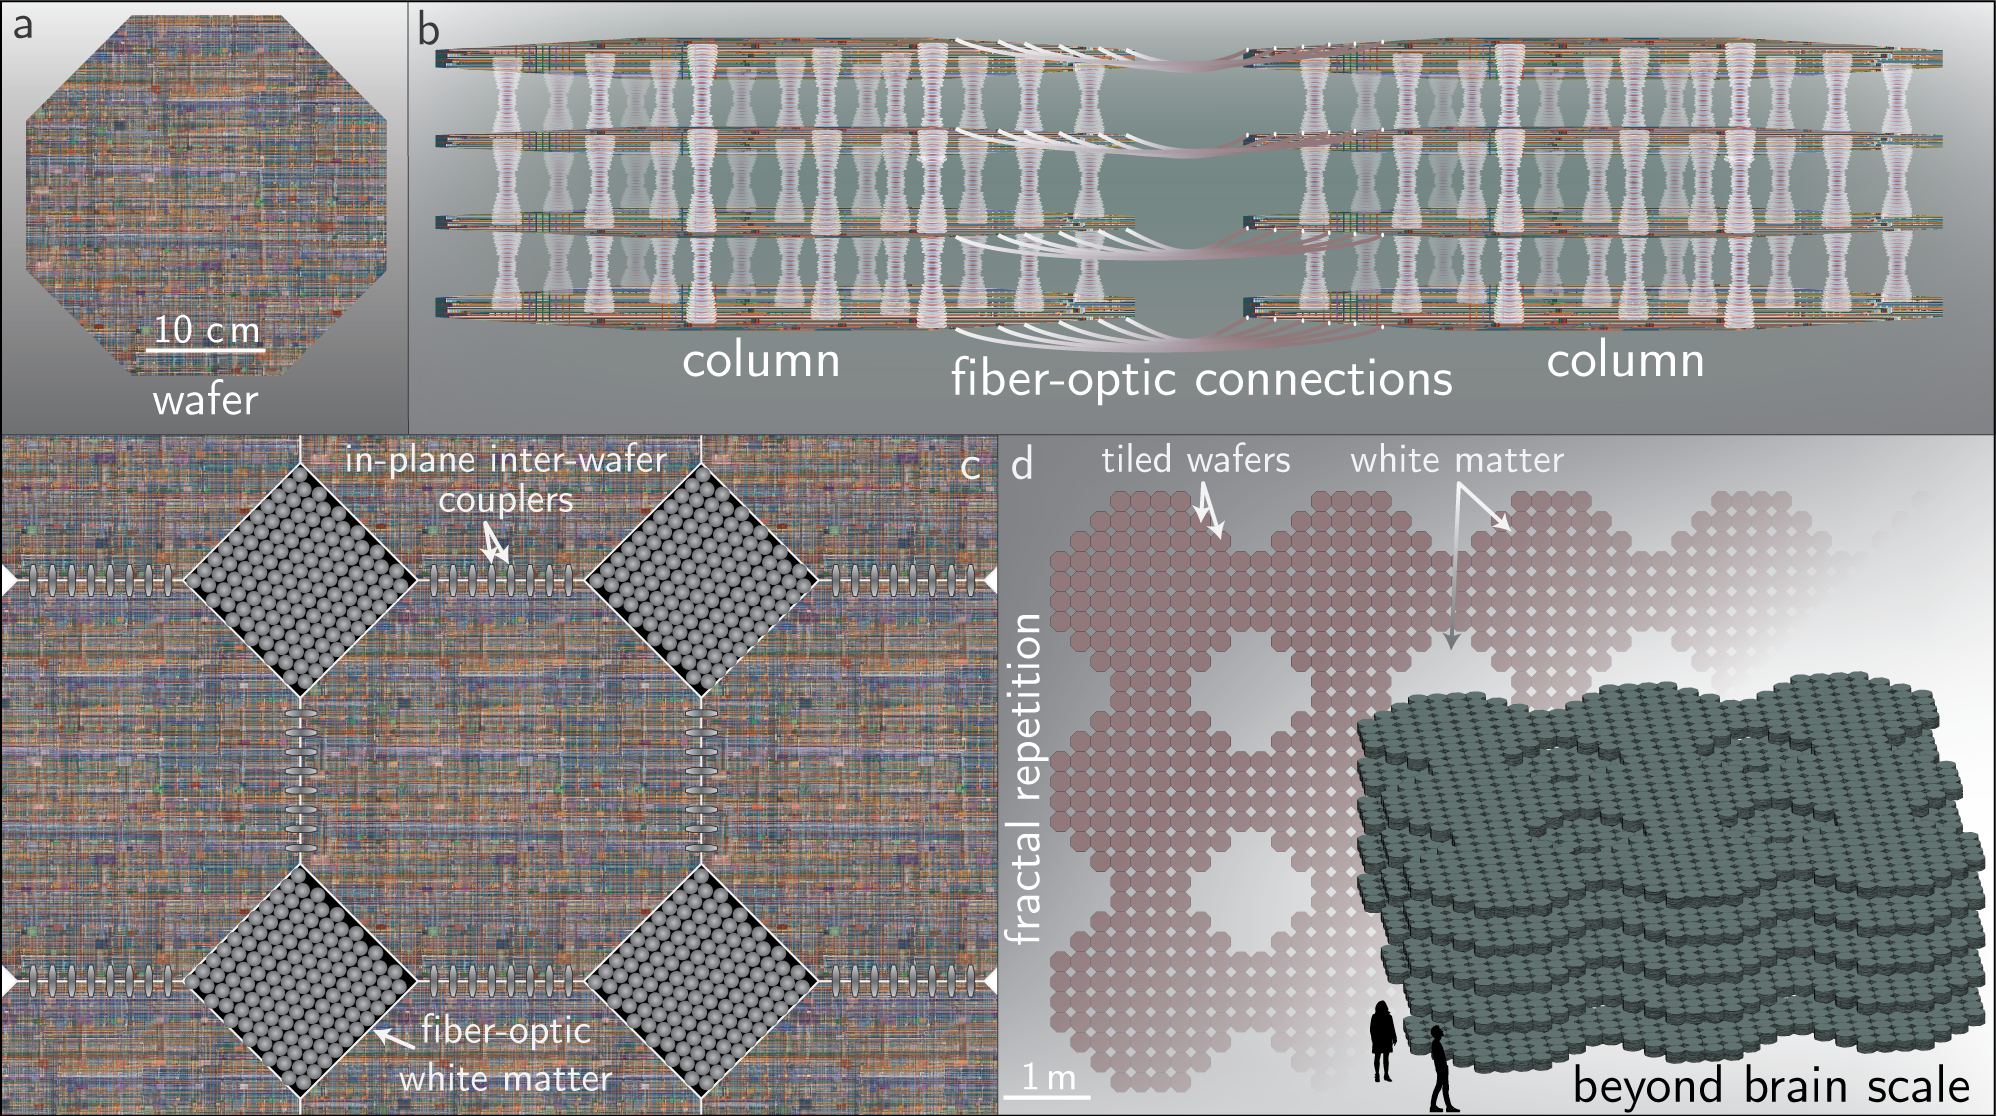
\includegraphics[width=17.2cm]{system.png}
    \caption{System. (a) (b) (c) (d)}
    \label{fig:system}
\end{figure*}

\subsection{Power consumption and cooling}

\subsubsection{Cooling Systems}
Cooling systems will be a key component to either platform. The ability to remove heat is necessary to maintain normal circuit operation. This is particularly dramatic for superconducting electronics, in which the devices will lose superconductivity if the temperature rises above the critical temperature ($T_c$). Pending a revolutionary development in high-$T_c$ materials, superconducting neuromorphic systems will rely on niobium ($T_c = 9.3$K) or a material with a similarly low $T_c$. Liquid helium (4.2K) is the cryogen of choice for such temperatures. Cooling systems will add significantly to the power consumption of superconducting electronics. The power efficiency of a refrigeration system is measured by its specific power (the reciprocal of the coefficient of performance) \textcolor{red}{(sounds like a bit of jargon to the uninitiated)} \cite{}. The specific power gives the number of watts consumed by the refrigeration system for every watt of heat removed. The theoretical limit for specific power, given by the Carnot limit, is $\frac{T_H - T_C}{T_C}$. For liquid helium temperature (4.2\,K), the Carnot limit demands that at least $74$\,Watts of refrigeration power are required to remove every watt of heat produced on-chip if the system is operated in a 300\,K ambient. State-of-the-art systems have reached specific powers as low $250$\,W/W. Auspiciously, the most efficient refrigeration systems also tend to have the highest heat loads. Heat loads as high as 10\,kW at 4.4K have already been demonstrated by commercially available systems. Note that throughout this paper, we assume a more conservative specific power of $1000$\,W/W, representative of the smaller scale cryogenic systems used in most laboratories today. Overall, it does not appear that cryogenic capability will be an insurmountable obstacle towards large-scale superconducting neural systems.

Heat leaks are another important consideration for superconducting systems. There are various mechanisms by which heat from the ambient environment can enter the cryogenic chamber, including conduction through structural components, thermal radiation, and leakage through I/O interconnects. This unwanted thermal power adds to the burden of the cryogenic system. In reference \cite{holmes2013energy}, it is estimated that heat leaks will consume about 10\% of the refrigeration power budget for a digital superconducting von-Neumann system. While this adds a standby power dissipation that would otherwise not exist in a superconducting system (aside from supporting semiconductor electronics for I/O, power supplies, etc.), it is not particularly important for the order of magnitude estimations desired in this paper.

\subsubsection{Power Limitations}
Modern supercomputers typically consume megawatts of power. Tianhe 2, for instance, requires 17.8\,MW for operation (and another 6.4\,MW for cooling) \cite{tolpygo2016superconductor}. If we thus assume a total power budget on the order of 10 MW, we can analyze the trade-off between average firing rate and the number of neurons. We assume 1\,fJ of optical energy is required to initiate a firing event at each synapse and plot the maximum average frequency spiking frequency for several different optical link efficiencies in figure \ref{fig:freq_size}.
\begin{figure}[H]
    \centering
    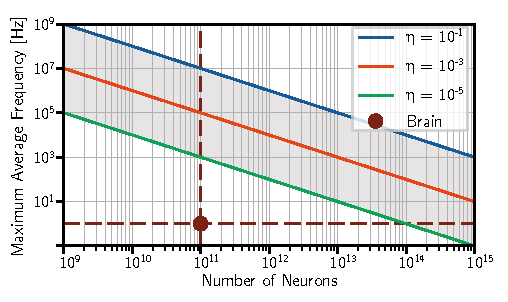
\includegraphics[scale=1]{Pow.pdf}
    \caption{Tradeoff between size and average spiking frequency for a population of optoelectronic neurons with a power budget of 10 MW. Fan-out is $10^3$ and the optical energy needed at each synapse is assumed to be 1\,fJ (accounting for cooling in superconductor case). This likely would correspond to the limits of either superconductor or semiconductor neurons.}
    \label{fig:freq_size}
\end{figure}

Power does not appear to be a limiting factor in achieving brain-scale and brain-speed optoelectronic networks. If the power resources of modern supercomputers were dedicated to a brain-scale optoelectronic neuromorphic system, average spiking rates on the order of 10 kHz appear feasible even with relatively inefficient optical links. Such a system, if designed to cultivate similar activity as the human brain, would enable brain-scale simulation with time accelerated by four orders of magnitude.

Another factor to consider is power density. There is a maximum power density that can be handled by heat removal systems for both the semiconducting and superconducting case. In the semiconductor case, high-performance computing routinely generates power densities of hundreds of watts per square centimeter \cite{tolpygo2016superconductor}. A theoretical limit of around 1\,kW/cm$^2$ is postulated in ref \cite{zhirnov2003limits}. In contrast, superconducting systems will be required to operate at significantly lower power densities. Roughly 1 W/cm$^2$ is a conservative limit on the on-chip power density that can be cooled with liquid helium \cite{tolpygo2016superconductor}. Interestingly, superconducting optical links appear to be capable of dissipating about three orders of magnitude less energy per bit, approximately cancelling out the limited power density requirements of superconducting systems in comparison with semiconductors. In practice, it might well be the case that mature, sophisticated synapses and neurons will occupy so much area that these power density limitations will be of no consequence. For instance, even with link efficiencies of $1 \times 10^{-4}$, a synapse would require a lateral dimension of less than 30\,$\mu$m for power density considerations to limit spiking to less than 1\,GHz. Section \ref{sec:instantiation} argued that synapses are not likely to be smaller than this. However, it should also be noted that optoelectronic systems will have extremely nonuniform power dissipation across the chip/wafer, with most of the power being dissipated at the light sources. A more in-depth analysis is required to see if heat removal will be an issue near the light-sources in particular. Concerns about local heating may be assuaged with layouts that sufficiently shield and/or separate thermally sensitive devices from the light sources.

\section{\label{sec:conclusion}Conclusion}

\textcolor{red}{(perhaps we should do something here to call attention to the key messages. perhaps they should be written concisely in bold--one or a few from each section.)}

\textcolor{red}{(the tone here is rosy, but quite a bit of what we're looking at indicates formidable challenges. the light source challenge is far from solved. monolithic 3d integration looks extremely advantageous, if not necessary for reaching brain scale, but this is not a slam dunk for either approach. memory is daunting. many in the semi world are looking to memristors, and speaking frankly, they are nowhere close to being able to implement the complex learning mechanisms of biology. the superconductor side may only appear better in this regard because we are naive due to the immature state of the effort. i'm inclined to try to capture the severity of the task before us, and also plainly state the challenges. And you accomplish this, i.e., ``Efficient, densely integrated light sources, waveguide-integrated detectors, local memory devices, and capable neuronal circuitry must all be consolidated onto a single platform.'' But this is followed by, ``Fortunately, excellent prior work has produced a variety of options on all of these fronts.'' We will need major progress on all these fronts, not to mention their combination. If the probability for each of these working on their own is $p_i$, the total probability is certainly less than $\prod_i p_i$. that could be pretty small. it is going to be very difficult to build more capable spiking neural systems than our brains. i don't mean to say the discussion is off the mark. it's not, and i like it a lot. these comments are about subtleties of the presentation.)}

The prospects of neuromorphic systems at the scale of the brain and beyond are tantalizing. The fan-out capability of optical communication, coupled with the computational power of electronic circuitry makes optoelectronic systems a promising framework for realizing these high ambitions. However, a number of hardware breakthroughs need to occur to make this vision a reality. \textcolor{red}{(should we summarize them in a table or some kind of visual form?)} Efficient, densely integrated light sources, waveguide-integrated detectors, local memory devices, and capable neuronal circuitry must all be consolidated onto a single platform. Fortunately, excellent prior work has produced a variety of options on all of these fronts. The great challenge is now to \sout{find the optimal} \textcolor{ForestGreen}{determine whether there is a} subset of technologies that can be practically interfaced \sout{together while maximizing performance} \textcolor{ForestGreen}{to achieve system feasibility}. Both semiconducting and superconducting technologies appear to \sout{hold the potential of supplying} \textcolor{ForestGreen}{offer} all the requisite devices for the application, and might even operate with surprisingly similar performance. However, the \textcolor{techological} paths toward achieving brain-scale systems \textcolor{ForestGreen}{with the two platforms diverge in important respects} \sout{are dramatically different for} , and we have attempted to outline the main advantages and challenges for each. 

Semiconductor optoelectronic neural systems can claim advantages in speed \textcolor{red}{(i'm not sure the text makes this case)}, \sout{fabrication infrastructure} \textcolor{ForestGreen}{technological maturity}, and room-temperature operation \sout{over their superconducting counterparts}. Spike rates in excess of 10 GHz are feasible \textcolor{red}{(with which light sources?)}, but static power dissipation is concerning for networks that are desired to operate at lower activity levels. Semiconductor receivers can potentially operate with extremely low energies per spiking event (sub femto-joule), making them a worthy competitor of superconducting single photon detectors. However, these low energy receivers require significant optical power \sout{out of} \textcolor{ForestGreen}{from} integrated light sources. To achieve biological-scale fan-out, either repeatering schemes (costing area and yield) or additional gain stages (costing power) will need to be included. In terms of neuronal computation, semiconductor neurons have already demonstrated impressive functionality and low-power operation that should be capable of integration with optical communication infrastructure, \textcolor{ForestGreen}{provided the long-standing challenges with CMOS-integrated light sources can be overcome}. Memory is a concern, but a variety of non-volatile memory solutions have seen extensive investigation. Still, a large-scale implementation of integrated memory with local plasticity update circuits is yet to be demonstrated \textcolor{red}{(could this offend someone working in that field?)}. Lastly, 3D integration of transistors, photodetectors, and memory will be an extremely challenging endeavor, given the necessity of high-temperature processing \textcolor{ForestGreen}{for dopant activation and contact metallization in semiconductor electronics}. The fabrication processes for mature semiconductor neural systems may prove to be \sout{extremely} \textcolor{ForestGreen}{prohibitively} complicated and heterogeneous, perhaps requiring different \sout{materials} \textcolor{ForestGreen}{processing strategies} for sources, detectors, and memories. \textcolor{ForestGreen}{If wafer-scale monolithic integration of these components cannot be achieved, and chip-scale die-stacking techniques are required, the outlook for achieving brain-scale systems becomes quite limited.}

Superconducting optoelectronic neural systems do not benefit as greatly from the maturity of the semiconductor industry, \textcolor{ForestGreen}{but can still make use of very similar foundry technologies, such as a 45-nm CMOS node processing 300-mm silicon wafers. The incorporation of superconducting electronics provides} several intriguing attributes. Namely, SNSPD receivers place nearly the theoretical minimum burden on integrated light sources. This is coupled with the \sout{known} improvements in efficiency for light sources operating at cryogenic temperatures. These two factors make the large-scale integration of light sources appear far more achievable than in the semiconductor case\textemdash perhaps even opening the door to silicon as an active optical material. Driving these light sources with superconducting electronics, however, has yet to demonstrated in \sout{a practical manner} \textcolor{ForestGreen}{with the performance required for this application; implementation of such a circuit remains a major open challenge}. Superconducting neuronal circuits appear just as capable of complex computation as their CMOS counterparts, but will likely need to be designed with serial biasing in order to scale. Additionally, \sout{the} some speed advantages present in superconducting electronics will be negated by the response time of SNSPDs \textcolor{ForestGreen}{, at least in regard to the speed of inter-neuronal communication. Computation within the neuron's dendritic tree leverages the speed of Josephson junctions for analog computation.} \textcolor{red}{(and light sources--how long does it take to make the requisite number of photons?)}, making \sout{operation} \textcolor{ForestGreen}{neuronal inter-spike intervals} above 1\,GHz unlikely. Memory seems to be a strength \textcolor{ForestGreen}{on the superconducting side of things}, \sout{however,} as superconductivity provides new avenues of storing synaptic weights. Loop memory in particular may be capable of implementing plasticity mechanisms that operate with only the signals produced through normal network activity. \textcolor{ForestGreen}{Caution is in order here, too, as these forms of synaptic plasticity mechanisms have scarcely been explored.} Finally, 3D integration \sout{appears more promising} \textcolor{ForestGreen}{may yield more readily} in the superconductor platform. \textcolor{ForestGreen}{The inconvenience of cryogenic cooling is a serious consideration, but power and heat removal estimations indicate this is unlikely to be a limiting factor for brain-scale systems.} \sout{and cooling systems are unlikely to be a limiting factor.} If all of these issues can be resolved, superconducting optoelectronic systems may actually require simpler manufacturing processes than the semiconductor approach, as the material ecosystem could potentially be relatively simple. Of course, superconducting foundries are far less developed than their semiconductor counterparts, which may negate these advantages in the near-term. \textcolor{ForestGreen}{Regarding speed limits, we must keep in mind that this upper firing limit is to be compared to the upper firing limit of pyramidal neurons engaged in gamma activity around 100\,Hz. Brain-scale systems with oscillations up to 1\,GHz would be a significant increase relative to present biological hardware. (something along those lines; the point is that 1GHz sounds slow compared to digital data rates, but for a spiking neural system of this scale it would be unimaginably fast)}

Finally, we would be remiss to paint the quest for neuromorphic supercomputing as only a question of hardware. The biological details of the inner workings of the brain remain an enigma of a magnitude eclipsed only by the \sout{question of how those inner workings could possibly give rise to} phenomena of \sout{the likes of} cognition and consciousness. Breakthroughs in neuroscience and algorithmic development (real spiking algorithms, not crude impersonations of back-propagation) will be required for the discussed hardware platforms to ever have any practical use. This summons the long-nagging chicken-or-the-egg question of whether we need hardware for algorithms or algorithms for hardware in neuromorphic computing. Fortunately, when you assume a 1000 year perspective on hardware, you might as well get started now, since you're going to need all the time you can get.

\textcolor{red}{(good outro, could use a little smithing)}

\bibliographystyle{unsrt}
\bibliography{bib}
\end{document}
